% !TEX TS-program = XeLaTeX
\documentclass{textolivre}

% used to create dummy text for the template file
%\usepackage{blindtext}
\definecolor{dark-gray}{gray}{0.35} % color used to display dummy texts
\usepackage{lipsum}
\SetLipsumParListSurrounders{\colorlet{oldcolor}{.}\color{dark-gray}}{\color{oldcolor}}

\journalname{Texto Livre: Linguagem e Tecnologia}
\thevolume{14}
\thenumber{1}
\theyear{2020}
\receiveddate{\DTMdisplaydate{2020}{07}{05}{-1}} % YYYY MM DD
\accepteddate{\DTMdisplaydate{2020}{08}{18}{-1}}
\publisheddate{\today}

\title{Práticas educativas ambientais na formação de educadores das infâncias}
\othertitle{Environmental educational practices in training children's educators}

\author[1]{Eliane Lima Piske}
\author[2]{Narjara Mendes Garcia}
\author[3]{Maria Angela Mattar Yunes}

\affil[1]{Universidade Federal do Rio Grande, Brasil. Email: \url{e.nanny@hotmail.com}}
\affil[2]{Universidade Federal do Rio Grande, Brasil. Email: \url{narjaramg@gmail.com}}
\affil[3]{Universidade Salgado de Oliveira, Brasil. Email: \url{mamyunes@gmail.com}}

%% Corresponding author
\corrauthor{Eliane Lima Piske}

%% DOI
\articledoi{10.35699/1983-3652.2021.25698}

%% Abbreviated author list for the running footer
\runningauthor{Piske et al.}

%\usepackage[backend=biber,style=abnt, ittitles]{biblatex}
%\DeclareLanguageMapping{brazil}{brazil-apa}
\addbibresource{article.bib}     
% use biber instead of bibtex
% $ biber tl-article-template
% $ pdflatex tl-article-template.tex

% set language of the article
\setdefaultlanguage[variant=brazilian]{portuguese}
\setotherlanguage{english}
% for langues that use special fonts, you must provide the typeface that will be used
% \setotherlanguage{arabic}
% \newfontfamily\arabicfont[Script=Arabic]{Amiri}
% \newfontfamily\arabicfontsf[Script=Arabic]{Amiri}
% \newfontfamily\arabicfonttt[Script=Arabic]{Amiri}
%
% in the article, to add arabic text use: \textlang{arabic}{ ... }

\begin{document}
\maketitle

\begin{poliabstract}
\begin{abstract}
Com o foco na perspectiva sistêmica, a formação permanente dos educadores ambientais das infâncias pode apresentar uma relação multidisciplinar potente entre as linguagens e a educação das crianças. O objetivo do estudo é investigar as práticas educativas ambientais de educadores das infâncias e suas perspectivas a partir de experiências em múltiplos contextos e culturas. A pesquisa é qualitativa e tem como base teórica o entrelace de conceitos da Biologia do Conhecer e da Bioecologia do Desenvolvimento Humano. A metodologia adotada foi a Inserção Ecológica, por meio da qual o pesquisador se insere nos espaços formativos para desenhar as oficinas de comunicação e reflexão, que foram inspiradas na Comunicação Não Violenta. Para a análise da produção de informações, utilizamos a ferramenta Sobek. Os resultados evidenciam que as trajetórias educativas são mobilizadas pela possibilidade da conversa(ação). Dessa forma, a contribuição do olhar bioecológico e a proposta experiencial das práticas educativas ambientais influenciam na constituição dos educadores das infâncias.

\keywords{Infâncias \sep Formação \sep Educadores \sep Linguagens \sep Bioecologia.}
\end{abstract}

\begin{english}
\begin{abstract}
Having a focus on the systemic perspective the permanent training of environmental childhood educators can bring a powerful multidisciplinary relationship between languages and children's education. The aim of this study is to investigate the environmental educational practices of childhood educators and their perspectives based on experiences in multiple contexts and cultures. The research is qualitative whose theoretical basis is the intertwining of concepts of the Biology of Knowledge and the Bioecology of Human Development. Ecological Engagement was the methodology through which the researcher included himself in the spaces of training to design the communication and reflection workshops. They were inspired in Non-Violent Communication. The analysis of information production was done with the support of the Sobek tool. Therefore the educational trajectories are mobilized by the possibility of conversation (action). Thus, the contribution of a bioecological view and the experiential proposal of educational environmental practices influence the constitution of children seducators.

\keywords{Childhood \sep Formation \sep Educators \sep. Languages \sep Bioecology.}
\end{abstract}
\end{english}
\end{poliabstract}


\section{Introdução}\label{sec-intro}
A relação multidisciplinar entre as múltiplas linguagens e a educação das crianças na formação docente é uma possibilidade para esmiuçar a Vertente Sistêmica da Educação Ambiental, a partir das expectativas dos educadores das infâncias. Isso está em consonância com o objetivo desse artigo: investigar as práticas educativas ambientais de educadores das infâncias e suas perspectivas, a partir das suas experiências em seus múltiplos contextos.

Os estudos teóricos foram pautados em autores como \textcite{maturana2011,rosenberg2006,brofen2011}. O embasamento metodológico contou com a participação em diferentes espaços formativos, seguido da Inserção Ecológica. O entrelace da formação docente com a Inserção Ecológica é capaz de atingir a produção de informações para construir as oficinas de comunicação e reflexão que foram desenvolvidas no Brasil e no Uruguai. Entrelaçar uma base sistêmica ambiental não é e nem poderia ser uma tarefa fácil, ainda mais se tratando de uma busca das expectativas dos educadores das infâncias para desenhar as estratégias para o levantamento das perspectivas e dos interesses das temáticas para a formação docente.

As microintervenções para formação docente foram inspiradas no Método da Comunicação Não Violenta (CNV), de \textcite{rosenberg2006}. No decorrer do artigo, os dados empíricos serão apresentados num emaranhado sistêmico ambiental, em que as partes totalizam a engrenagem dos vértices para apresentar as perspectivas dos educadores das infâncias na educação das crianças. Os conhecimentos compartilhados a partir das experiências são uma possibilidade para explanar os conceitos: linguagens, infâncias, crianças e formação docente; saberes que não são imperativos, mas que compõem a identidade acerca do olhar, dos objetos, dos discursos, enfim, das conversas, do linguajar e das emoções que constituem as educações nos múltiplos contextos. Neste ínterim, educação é a totalidade dessas percepções em diversos cenários, sendo o contexto ecológico que vai diferenciar, se é um espaço formal, informal ou não formal. 

A triangulação dos espaços possibilitou abalizar a proposta, que será apresentada em subitens, capaz de explanar a conversa(ação) firmada com os educadores das infâncias de diferentes contextos ecológicos microssistêmicos. A nuance sistêmica é a evidencia que comprova a necessidade da formação docente ser construída a partir das experiências. Isso será apresentado nas considerações preliminares, seguido da metodologia da pesquisa. O destaque para a análise da produção de informações e os resultados serão expostos com a utilização da ferramenta Sobek \cite{epstein2017,couto2015}, um aplicativo mantido e desenvolvido pelo Programa de Pós-Graduação em Informática na Educação, na Universidade Federal do Rio Grande do SUL (UFRGS), Brasil, e por fim, as considerações finais do estudo.

\section{Considerações preliminares}\label{sec-consideracoes}
Educar é algo que fazemos no e com o viver pelas palavras de \textcite[p. 185]{maturana2009}: “vivemos tudo o que vivemos como válido no momento de vivê-lo e, nesse viver, tratamos como válidas as coerências operacionais que surgem como constituindo o espaço relacional que emerge com nosso viver”. Ser e estar em permanente movimento é o que move nossa existência, a ação faz (e é) parte desta conversa que transformou a formação docente pela oportunidade de vivenciar a linguagem da comunicação não-violenta \cite{rosenberg2006}. Segundo \textcite[p. 96]{brofen2011}: ``aqui estamos lidando com o organismo como um todo, possuindo características genéticas, fisiológicas, emocionais, cognitivas e sociais que funcionam distintamente em meios diferentes e em contextos amplos. Aspectos da infância, no entanto, que vão além das características genéticas e biológicas''.

De acordo com \textcite[p. 32]{maturana2011}: “todo fazer é um conhecer e todo conhecer é um fazer”. A aceitação é o fazer, então operar a teoria é justamente essa a ideia, de afinidade, de conversa, no sentido de relacionar as coisas pelo respeito ao conviver. Segundo \textcite[p. 31]{maturana1998}: “sem aceitação e respeito por si não se pode aceitar e respeitar o outro, e sem aceitar o outro como legítimo outro na convivência, não há fenômeno social”. Tal ideia vem ao encontro da CNV, no sentido de embasamento teórico metodológico transversal diante da pesquisa. O processo da CNV tem uma metodologia muito prática que é a comunicação, o reconhecimento do sentimento, das necessidades e dos pedidos. Conforme \textcite[p. 25]{rosenberg2006}: “para chegar ao mútuo desejo de nos entregarmos de coração, concentramos a luz da consciência em quatro áreas, às quais no referimos como os quatro componentes do modelo da CNV”.

Com a breve explanação da Vertente Ambiental Sistêmica, se demonstra que ambos os autores constroem e ressignificam a arte do educar como base do desenvolvimento humano. Podemos constatar que \textcite{maturana2011,brofen2011,rosenberg2006} trazem as possibilidades em aliar e discorrer sobre as questões ambientais pela totalidade de atuações, pela origem do mundo, do conhecer, da natureza e do viver, sendo estas as bases bioecológicas da compreensão humana. Os autores citados defendem os conhecimentos no contexto amplo, pela preservação natural e pelas questões dos ambientes em sua totalidade. Segundo \textcite[p. 195]{maturana2011}: “falamos em conhecimento toda vez que observamos um comportamento efetivo (ou adequado) num contexto assinalado. Ou seja, num domínio que definimos com uma pergunta (explicita ou implícita) que formulamos como observadores”. Portanto, isso está em sintonia com a definição dos elementos processo-pessoa-contexto-tempo (PPCT) para o desenvolvimento humano \cite{brofen2011} e dos quatro componentes da CNV: observação, sentimento, necessidade e pedido \cite{rosenberg2006}. 

O modelo de sociedade a que pertencemos foi constituído por nós, seres humanos, pela capacidade de associar o plano da ação com o respectivo fazer. Conforme \textcite[p. 91]{carvalho2012}: “cada sociedade humana, a mesma sociedade em diferentes momentos de sua história, e diferentes grupos dentro da mesma sociedade têm suas próprias concepções sobre o que é um bebê, uma criança, um ser humano”. Nenhum outro ser vivo tem essa capacidade, esse conjunto de circunstancialidade que se desenha num tempo e se constituem na memória e complexidade dos sistemas \cite{piske2019}. 

A conjectura sistêmica é latente já que é uma engrenagem de múltiplos elos que precisam estar e permanecer em sintonia, para que o trabalho das peças movimente o todo. Sendo assim, a máquina precisa dos componentes para seu funcionamento e é necessário conhecer esses mecanismos para que elas trabalhem. Nós, seres vivos, também necessitamos de uma organização:

\begin{quote}
O fato de que o conhecer seja o fazer daquele que conhece está enraizado na própria maneira de seu ser vivo, em sua organização. Sustentamos que as bases biológicas do conhecer não podem ser entendidas somente por meio do exame do sistema nervoso. Parece-nos necessário compreender como esses processos se enraízam na totalidade do ser vivo \cite[p. 40]{maturana2011}.
\end{quote}


Temos que compreender a organização dos seres vivos em sua totalidade que são experienciados: cérebro, linguagem e afeto, na lógica social e no contexto concreto. Não se deve esquecer que as perspectivas têm influências nas questões culturais e nos contextos sociais, que são as bases bioecológicas do desenvolvimento humano. Conforme \textcite[p. 31]{gomes2013}: “em nossa opinião, grande desafio que se apresenta hoje à sociedade, em geral, e à educação, em particular, é o equilíbrio das relações entre o coletivo e o individual, o público e o privado, o pensamento flexível e o pensamento único/homogêneo”. Somos nós quem apresentamos identidade para o lugar no momento que (re)significamos este para a nossa constituição, enquanto sujeitos pertencentes a um contexto sócio-biológico-sistêmico, formado pela cultura, a biologia e a complexidade do tempo: tríade interativa.

É preciso reafirmar também que os seres vivos estão interligados com o mundo, por isso a importância das interações bioecológicas entre os condicionantes. De acordo com \textcite[p. 67]{maturana2011}: “cada vez que, num sistema, um estado surge como modificação de um estado prévio, temos um fenômeno histórico”. É necessário compartilhar dos pontos de vista: cultural, afetivo e social ao qual pertencemos, construir e poder modificar o espaço das ações que precisam e devem ser em sua totalidade de atuações.

A visão sistêmica de mundo pelo ser educador das infâncias (EI) possibilita encontrar a sintonia para que as crianças e os adultos sejam mais afetuosos. As pessoas não são e/ou estão isoladas do contexto. É preciso entender que tudo está relacionado, que não temos como tirar o indivíduo do seu lugar, pois ele é o ambiente, e este forma sistemas. Afinal, o que define a perspectiva sistêmica? A visão sistêmica é uma forma de olhar e atuar no mundo, de maneira que podemos perceber as conexões entre os sujeitos e o ambiente. Os sistemas são níveis de entendimento, as extensões em que podemos dimensionar pelo ser e não pelo ter, são fundantes das perspectivas dos educadores ambientais das infâncias em relação à linguagem pelo processo com as educações, que estão implicadas pelas abordagens sistêmicas nos múltiplos contextos, o que nos possibilitou chegar à metodologia do estudo.



\section{Etapas e metodologia da pesquisa: abordagens sistêmicas ambientais}\label{sec-etapas}
A Teoria do Conhecer é a questão do pesquisador implicado na própria teoria, compreendendo que tudo que é dito é falado por alguém e o observador pode ser ele mesmo quem está sendo observado. \textcite{maturana2011} explicam que todo o observador que se pergunta é um pesquisador em sintonia com o que compartilha. O modelo PPCT de \textcite{brofen2011} fundamenta os quatro passos da CNV. Em todo o comportamento humano é necessário associar os elementos, em que o olhar bioecológico faz a diferença para a realização da investigação, de cunho qualitativo. 

Por isso, partimos do pressuposto de que o ponto de análise é o olhar bioecológico, que integra a armação metodológica: a Inserção Ecológica do pesquisador nos contextos ecológicos microssistêmicos \cite{piske2018c,koller2016,silveira2009}, seguida da participação em diversos espaços formativos. A triangulação da Inserção Ecológica, a participação nos espaços formativos e a criação do Curso Educação Ambiental das Infâncias foram necessários para desenhar as microintervenções de comunicação e reflexão. A construção de significados entre os educadores das infâncias e o meio a partir de suas interações e experiências na educação das crianças foram baseadas numa perspectiva indissociável dos quatro elementos – PPCT. 

As dimensões construtivas da vertente metodológica sistêmica possibilitaram o olhar bioecológico no estudo: processo que é a educação pelas relações proximais, o tempo que é a trajetória educativa, as pessoas que são os educadores das infâncias e as crianças e os contextos que são os ambientes ecológicos microssistêmicos, ou seja, os lugares próximos, onde as relações e atividades face a face são estabelecidas.  

O método adotado na pesquisa teve como propósito apresentar estratégias claras, coerentes e operativas na formação de educadores das infâncias, uma vez que se dá em muitos contextos do mapa ecológico da criança, desde os mais distais (macro, exo e mesossistemas), e sobressaindo-se no mais proximal, o microssistema. Para dar uma compreensão bioecológica das perspectivas dos educadores das infâncias sobre a educação das crianças, a inserção ecológica foi realizada. Isso quer dizer que acompanhamos a situação cotidiana do trabalho dos educadores das infâncias por meio de uma imersão no contexto, com anotações das observações naturalísticas em diário de campo. Na sequência, foi realizado o contato mais proximal com as educadoras por meio da participação em diversos espaços formativos.  

Neste implexo movimento sócio-biológico-sistêmico, foi necessário que os pesquisadores colocassem uma armação de óculos contendo a lente ecológica para enxergar os acontecimentos a partir do conteúdo bioecológico, qual seja compreender como os contextos ecológicos microssistêmicos se apresentam e não a partir de preconceitos e/ou julgamentos. Sendo assim, a metodologia foi desenhada ao contemplar as dimensões que fizeram (foram) a capacidade reflexiva para abalizar a pesquisa qualitativa, em que as observações naturalísticas e o diário de campo foram instrumentos inseparáveis do estudo. A seguir, serão compartilhados e discutidos os detalhes mais relevantes do processo investigativo: os contextos, as infâncias, os educadores, as crianças, os procedimentos de interação e o levantamento das informações, a análise dos dados e as respectivas reflexões.

As infâncias são sempre os modos como os educadores entendem como as crianças devem viver naquele período de vida, as infâncias foram construídas ao longo da modernidade. Já as crianças são as pessoas que, de acordo com o Estatuto da Criança e do Adolescente \cite{eca1990}, tem de zero até doze anos incompletos. E os educadores das infâncias são aqueles que compõem a equipe intersetorial, entendida aqui como todos os profissionais da educação (estudantes de licenciatura, monitores, cuidadores, educadores sociais, recreacionistas, professores de educação física, pedagogos, psicólogos, dentre outros), assim como as figuras parentais, incluindo na expressão quaisquer cuidadores, sejam pais biológicos, adotivos, sociais e/ou avós \cite{piske2019}.

A partir de então, serão esmiuçadas as duas fases da investigação: a inserção ecológica nos contextos ecológicos microssistêmicos \cite{piske2018c,koller2016,silveira2009} e a participação em diversos espaços formativos, como congressos, cursos, oficinas, dentre outras possibilidades da formação docente, tanto na modalidade presencial quanto à distância. As abordagens mencionadas possibilitaram a criação de oficinas de comunicação e reflexão que foram inspiradas no Método da Comunicação Não Violenta \cite{rosenberg2006}. 

Apresentamos as etapas e os instrumentos do estudo: inserção ecológica; observações naturalísticas; gravações de áudios; diário de campo; participação nas formações docentes; encontros com a Bolsista de Iniciação Científica; as oficinas de comunicação e reflexão e os termos: Termo de Consentimento Livre e Esclarecido - TCLE e o Termo de Assentimento -- TA \cite{Missio2018}. Os princípios éticos foram essenciais para o desenvolvimento da pesquisa e os educadores das infâncias tiveram que autorizar a divulgação das informações, através de TCLE. Foram assinados o TA pelas crianças, que também tiveram a opção de escolher o desenho como forma de assentir, ambas concordaram em participar do estudo.

No decorrer da investigação, elucidaremos cada um dos passos, assim como as respectivas informações. Retomando a explicação, enfatizamos: os pesquisadores precisaram colocar a lente ecológica para enxergar os acontecimentos a partir do viés bioecológico. Precisaram entender quem eram as pessoas, quais eram as representações sociais que ali estavam colocadas e não foi somente a partir do que os pesquisadores interpretaram, todavia, foi necessário construir outra lente para aquilo que estavam observando, como os contextos microssistêmicos realmente se apresentam. 
As estratégias de conversa(ação) com os educadores das infâncias ao (re)significar o olhar bioecológico foram a base da investigação, uma possibilidade da Inserção Ecológica \cite{piske2018c,koller2016,silveira2009} com a participação em diferentes espaços formativos, abordagens associativas que contemplam a ideia do pesquisador misturado, já que numa pesquisa qualitativa não tem como ser neutro. A lente ecológica e o olhar bioecológico não são iguais, mas têm bastantes similaridades. Consideramos que o termo expõe o detalhamento ou a escolha do ponto de análise de uma condição ou situação presente no ambiente, ou seja, nos contextos ecológicos microssistêmicos. 

Neste ínterim, entrou em cena o olhar bioecológico: uma evidência metodológica para interpretar melhor as circunstâncias, como realmente são as coisas. A lente ecológica é a forma como tentamos buscar o viés bioecológico, que é algo para além daquilo que o pesquisador interpreta. Vamos imaginar uns óculos, um dispositivo para ampliar a visão, a armação dos óculos contém duas lentes oftálmicas e uma armação. Sendo assim, como vamos conseguir o olhar bioecológico? A resposta é simples: tendo em vista a integralidade das dimensões -- PPCT -- olhar bioecológico. 

Em síntese, a lente que é bioecológica enxerga as pessoas, os contextos que eles estão, a influência do tempo e os processos implicados ao serem construídos na totalidade dos elementos: o olhar bioecológico de cada um. Todavia, é preciso contemplar os quatro níveis: pessoa, processo, contexto e tempo, o mapa bioecológico. O olhar bioecológico pode variar, já que cada um tem o seu próprio olhar, o que é importante em termos de pesquisa sob escopo da Inserção Ecológica. Assim, quanto mais pessoas para compartilhar as impressões, mais acurada será a Inserção Ecológica. 

No que se refere à diferença entre o olhar e a lente, temos a seguinte proposta reflexiva: a armação dos óculos contém duas lentes e é necessária para ampliar a visão. Entretanto, para enxergar a armação dos óculos requer lentes adequadas para, no caso, podermos visualizar apropriadamente os contextos ecológicos microssistêmicos. Apesar da lente também ser individual ela precisa atender as especificidades para prover o olhar. Numa tentativa de síntese na pesquisa, as lentes são as teorias sistêmicas: Bioecologia do Desenvolvimento Humano \cite{brofen2011}, a Comunicação Não-Violenta \cite{rosenberg2006} e a Biologia do Conhecer \cite{maturana2011}, uma forma de contemplar para poder enxergar. Já o olhar bioecológico guiou a metodologia prática que usamos para poder chegar até a lente, no caso, o embasamento sistêmico transversal durante o estudo, resultando na possibilidade para desenhar as oficinas de comunicação e reflexão.

Os estranhamentos aparecem como parte das problematizações da lente bioecológica. Devemos entender que estamos colocando óculos que contém as lentes para a inserção nos diferentes contextos ecológicos microssistêmicos. Para tal, é necessário visualizar os contextos microssistêmicos a partir de outra visão: do olhar bioecológico. O olhar do pesquisador precisa ser algo que não esperamos. Colocamos a lente para tentar enxergar o(s) contexto(s) microssistêmico(s), mas na condição de pesquisadores não temos como saber o que vamos encontrar. Assim, o mais desafiador é: quais seriam as representações que iramos levar daquela experiência? Não podemos esquecer os aspectos a priori e que não podemos desconsiderar que os pesquisadores são os sujeitos participantes, pessoas que estão em interação no contexto e que percebem os sentimentos, estes, que para a CNV, são a alegria, a raiva, o medo e a tristeza.

Nesse aspecto, foi fundamental estabelecer uma conversa legítima com os educadores ao refletir com eles a premência da real democracia das infâncias nos contextos ecológicos microssistêmicos. A valorização positiva das crianças foi a possibilidade de refletir condutas e ações como centrais em seus próprios processos, o eco das vozes sensíveis ao ser, fazer e estar em constante (re)pensar as atuações a partir das experiências nos ambientes. Sendo assim, foi necessário construir o mapa ecológico dos contextos, enquanto nós, pesquisadores(as) que fizemos parte do(s) ambiente(s) pesquisado(s), estávamos em interação com os sujeitos. 

No sentido de embasamento transversal, defendemos a ideia de que a lente deve ser entendida como uma teoria, e que precisamos colocá-la em foco. Na metodologia da pesquisa da Vertente Sistêmica em Educação Ambiental \cite{piske2018b,piske2019} discorre que é preciso ter a lente bioecológica, embasada transversalmente para alcançar a base sistêmica: o olhar bioecológico. Podemos fazer a comparação da lente com a ideia da lente de uma máquina fotográfica, sendo o primeiro passo para entendermos esse olhar mais aprofundado.

O olhar bioecológico parte de quatro dimensões, pessoa, processo, tempo e contexto, e é a forma de contemplar a realidade, que é o PPCT. Partindo do pressuposto de que a lente bioecológica tem afinidade com a forma que cada pessoa enxerga, a diferença das perspectivas dos sujeitos é a maneira com que cada um percebe determinado acontecimento, pois essa lente tem como base as experiências individuais. Então, todos nós temos o olhar bioecológico, porém cada um de nós vai desenvolver uma lente bioecológica. Comparando à lente de uma câmera fotográfica, para um melhor entendimento, o foco dessa lente irá depender do tipo de máquina que vai comportá-la, quer mais absoleta ou mais moderna. 

A forma como enxergamos a realidade tem como base as individualidades, as experiências e as relações; já o olhar bioecológico tem afinidade com as dimensões para aquilo que olhamos. Fazendo a analogia com a câmera, mesmo que duas pessoas tenham a mesma máquina e são indicadas a fotografarem o mesmo contexto, certamente o resultado serão fotos distintas, pois cada uma delas tirará fotos de diferentes ângulos, diferentes focos e diferentes percepções. Entretanto, às vezes o olhar está muito mais focado para a pessoa do que o contexto, no qual a pessoa está.

No mesmo sentido, uma das dimensões que também podemos estabelecer a comparação usada anteriormente é que o tempo também age nesse processo como grande influente. A lente de uma máquina, por exemplo, evolui na sua resolução, ganha forma tecnológica, isto é, se modifica de acordo com o tempo, dentro de um contexto, pois, independente da lente, é necessário que as pessoas enxerguem as dimensões de forma indissociável, que tenham o olhar bioecológico.

A Inserção Ecológica em contextos ecológicos microssistêmicos foi realizada para conhecer os ambientes e as perspectivas dos EI com as crianças. Paralelamente com a participação em espaços formativos foram utilizadas na fase inicial do levantamento da produção de informações as possibilidades para desenhar as oficinas de comunicação e reflexão. Para o registro das observações naturalísticas contamos com o diário de campo, o registro fotográfico e as gravações dos áudios.

Neste primeiro momento de diagnóstico foram analisados os discursos dos educadores das infâncias nos contextos ecológicos microssistêmicos. Conforme mencionado, a Inserção Ecológica priorizou que os pesquisadores se aproximassem das pessoas para conhecer as peculiaridades dos contextos microssistêmicos e estabelecer relações, tendo o olhar cuidadoso ao integrar o tempo pelos processos proximais, uma função diagnóstica a priori, nas concepções do Modelo Bioecológico do Desenvolvimento Humano \cite{brofen2011}.



\section{Os contextos pesquisados e suas representações}\label{sec-contextos}
A Inserção Ecológica foi realizada em três contextos ecológicos microssistêmicos, sendo uma escola de anos iniciais da rede pública, uma escola de educação infantil e uma instituição não governamental. Foi possível conhecer as pessoas pelas observações realizadas em diferentes horários, turnos e dias, dentre vários momentos. A Inserção Ecológica \cite{piske2018c,koller2016,silveira2009} é um método de pesquisa qualitativa que prioriza que investigadores estabeleçam interações proximais com os participantes da pesquisa para melhor compreender os processos, o tempo e suas ações cotidianas. As Inserções Ecológicas começaram no mês de março de 2017 e terminaram em dezembro de 2018, o tempo da produção de informações a partir das Inserções nos múltiplos contextos.

Nesse estudo, tivemos a participação de uma bolsista de Iniciação Científica, colaboradora indispensável à investigação. Esta ficou responsável por realizar anotações em diário de campo. Inicialmente, construímos um guia para contribuir com a Inserção Ecológica da bolsista nos múltiplos contextos e organizamos um roteiro para investigar as perspectivas dos educadores das infâncias a partir das experiências compartilhadas com as crianças nos contextos ecológicos microssistêmicos. Vale mencionar que alguns envolveram mais conteúdos e outros mais valores, os princípios e as educações pelas trajetórias educativas.

A Inserção Ecológica como estratégia teórico-metodológica pela Vertente Sistêmica em Educação Ambiental foi uma possibilidade para constatar que não precisamos concordar para legitimar o outro. Muitas vezes estamos dentro dos contextos ecológicos microssistêmicos e não concordamos com a atitude e/ou a opinião de uma pessoa, mas nem por isso deixamos de respeitar o outro. Sendo assim, como os pesquisadores podem se inserir nos contextos ecológicos ao legitimar o(s) outro(s)? A Inserção Ecológica do pesquisador no ambiente a ser investigado contribuiu para o entendimento do desenvolvimento humano e dos processos que estão (são) implicados ao estudo. 

O desenvolvimento neste caso é visto como o resultado da multiplicidade de processos de interações recíprocas entre as pessoas e dessas em seus contextos ecológicos microssistêmicos. A partir deste método, o pesquisador estabeleceu interações significativas com as pessoas no ambiente estudado. Assim, as influências mútuas entre o pesquisador e as pessoas se constituem em processos proximais \cite{brofen2011}. Os processos proximais são entendidos enquanto formas particulares de interação entre o organismo e o ambiente e que ao longo do tempo se operam de formas progressivamente mais complexas. Estes processos tanto podem ser conduzidos por relações interpessoais, bem como pela interação da pessoa em desenvolvimento com os objetos e os símbolos, sem a presença de outras pessoas. 

Sendo assim, quando olhamos o que o outro fala (faz) é mais fácil do que (re)pensar nossas atuações? Como pensar a educação sem refletir sobre os contextos ecológicos microssistêmicos? Bronfenbrenner com o trecho a seguir possibilita a reflexão: 


\begin{quote}
Descobri na releitura que havia algumas tendências na ciência do desenvolvimento nessa história que passaram despercebidos. Recordo-me, a esse respeito, de uma fábula bastante conhecida (...). Na qual um homem está falando de sua visita a um jardim zoológico e todas as criaturas que lá viu: “as pequenas moscas e besouros, borboletas e insetos, e joaninhas com uma cabeça não maior do que um alfinete. Que maravilha!” “E você viu o elefante?”, perguntou seu amigo. “Ah, eles têm um lá? Acho que eu devo ter perdido o elefante.” \cite[p. 95-96]{brofen2011}.   
\end{quote}

O olhar bioecológico pode variar de acordo com a perspectiva. Conforme já mencionado nesse texto, quanto mais pessoas para compartilhar as impressões maior será a qualidade da Inserção Ecológica do pesquisador nos contextos ecológicos microssistêmicos. A reflexão é diferente da ação, pois o ato de olhar para nós mesmos a partir daquilo que pensamos até chegar a modificação da atuação não é igual. Muitas vezes, agimos centrados nas ações e não na reflexão. Algumas vezes, falamos sobre a experiência depois que ela passou. É o momento em que o educador das infâncias percebe que aquela determinada ação precisa ser revista, ser (re)olhada, (re)analisada, (re)pensada e problematizada. Precisamos estar neste processo de permanente reflexão sobre a própria ação, para ter novos desempenhos. A Inserção Ecológica contribuiu para reforçar e gerar essas constatações.  

Bronfenbrenner (2011) afirma que há reciprocidade nas relações de desenvolvimento humano. O que acontece nos ambientes, os problemas, os conflitos e/ou as soluções vão de certa maneira ser uma experiência e vão interferir no processo educativo que é à base do desenvolvimento humano. A Abordagem Bioecológica do Desenvolvimento Humano, proposta por \textcite{brofen2011}, contempla a ideia de que o desenvolvimento humano acontece de maneira ampla e promove as interações e relações das pessoas com ele mesmo, com o outro e com os ambientes. \textcite{brofen1996} explica que a afetividade, as relações e os afazeres devem ter um equilíbrio de poder e reciprocidade entre e com os contextos resultantes da abordagem. 

De acordo com a Ecologia do Desenvolvimento Humano de \textcite{brofen1996}, o ambiente é composto por contextos ecológicos, desde os mais proximais até os mais distantes, situados em lugares e tempo histórico. A terceira dimensão do desenvolvimento humano é o contexto que compreende quatro níveis ambientais, denominados: microssistema, mesossistema, exossistema e macrossistema. O microssistema é representado por contextos em que ocorrem interações face-a-face pela pessoa em desenvolvimento, aqueles ambientes mais próximos, o mesossistema é a inter-relação entre os microssistemas, já o exossistema é um contexto ecológico que envolve ambientes não freqüentados ativamente pela pessoa e/ou grupo, mas que também desempenham influências indiretas ao desenvolvimento humano. Finalmente, o macrossistema que é composto pelo conjunto de ideologias, de valores, de crenças, das religiões, das formas de governo, das políticas públicas e das culturas presentes no cotidiano das pessoas que influenciam no desenvolvimento humano \cite{brofen1996,piske2019}. A representação dos níveis ambientais é apresentada no desenho, que foi a inspiração para a criação do logo do Grupo de Estudos Ecoinfâncias, mas com ele podemos visualizar a pessoa que está no centro da representação, mas que sofre a influência, conforme podemos visualizar na \Cref{fig-fig01}.

\begin{figure}[h!]
 \centering
 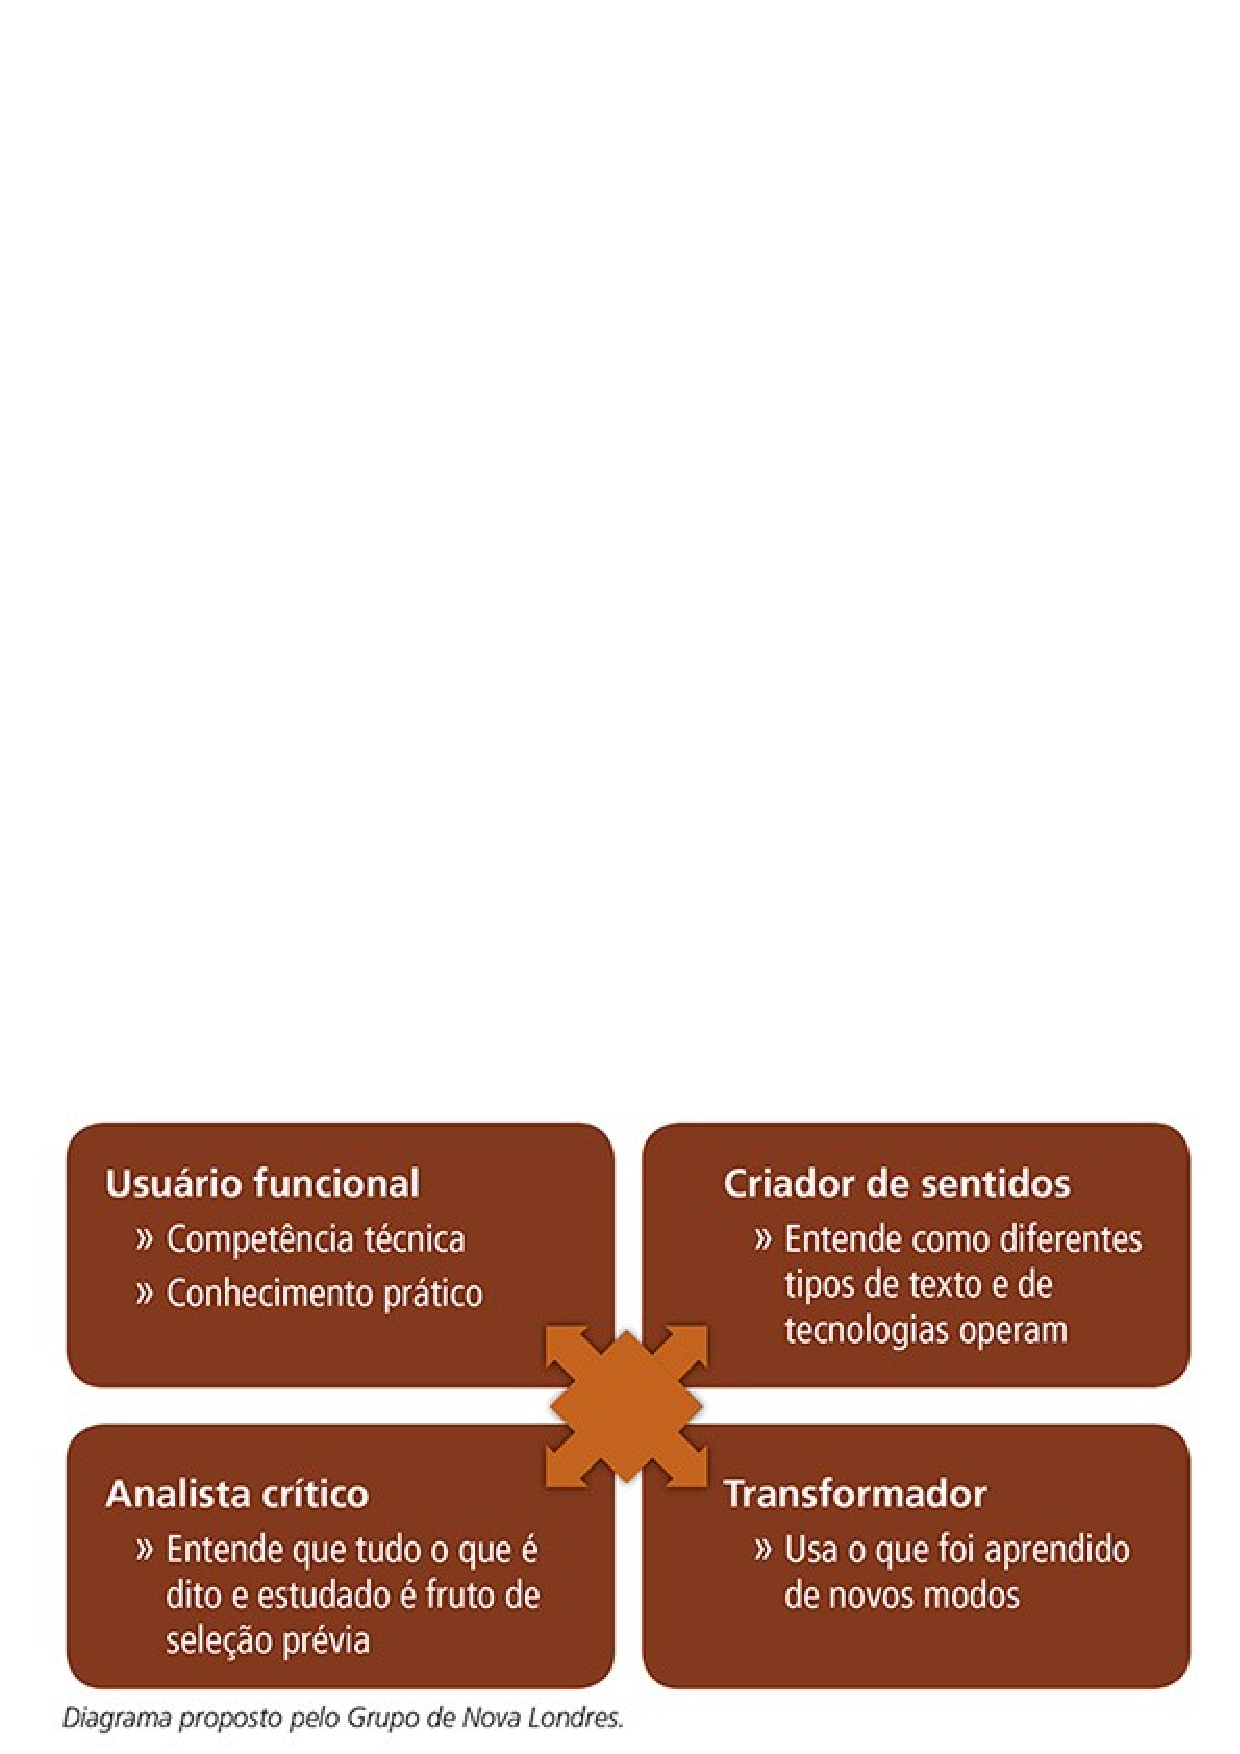
\includegraphics[width=0.5\textwidth]{figure01.png}
 \caption{contextos ecológicos desde os mais próximos até os mais distantes.}
 \label{fig-fig01}
 \source{Felipe, 15 anos.}
\end{figure}

Nesse sentido, o modelo explicativo do desenvolvimento humano deve ser composto e compreendido na ótica de quatro dimensões inter-relacionadas: processo, pessoa, contexto e tempo (PPCT). Chamamos a atenção para a contribuição da Inserção Ecológica, que envolve os quatro elementos na pesquisa. A Inserção Ecológica \cite{silveira2009,piske2018c,koller2016} é a possibilidade de levar em consideração as ideias e percepções do pesquisador como parte do contexto investigado, pois não existe neutralidade nesse processo de percepção e na interpretação dos saberes ambientais.

No mesmo período da Inserção Ecológica, participamos das formações docentes em diferentes espaços formativos, tanto na modalidade a distância como presencial para conhecer as práticas e os discursos dos educadores das infâncias, conforme podemos visualizar na \Cref{tbl-tabela-01}.  

\setlength\LTleft{-1in}
\setlength\LTright{-1in}
\begin{small}
%\begin{longtable}{p{3cm}p{3cm}p{3cm}p{3cm}}
%\begin{longtable}{p{0.25\textwidth}p{0.25\textwidth}p{0.25\textwidth}p{0.25\textwidth}}
%\begin{longtable}{*{4}{p{0.27\textwidth}}}
\begin{longtable}{
    >{\raggedright\arraybackslash}p{0.18\textwidth}
    >{\raggedright\arraybackslash}p{0.18\textwidth}
    p{0.33\textwidth}
    p{0.37\textwidth}
    }
%\begin{table}[htpb]
\caption{Formação docente.}
\label{tbl-tabela-01}
%\begin{tabular}{p{3cm}p{3cm}p{3cm}p{3cm}}
\\
\toprule 
PARTICIPAÇÃO NOS ESPAÇOS FORMATIVOS & CIDADE/PERÍODO & MOMENTO(S) & PARTICIPANTES/ MINISTRANTES \\
\midrule
Turmas de graduação. Foi realizado nas disciplinas de Estágio I e Atividade de Docência II, 
ambas as disciplinas do Curso de Pedagogia Licenciatura pela Universidade Federal do Rio Grande- FURG. & 
Rio Grande \newline Março de 2017 até novembro de 2017 & 
O estágio de docência compreendeu atividades presenciais e a distância tendo a educação das infâncias como temática. &
Na disciplina Estágio I, participaram 32 estudantes. Na disciplina Atividade de Docência II participaram 29 estudantes. 
O Estágio de Docência resultou em um artigo completo apresentado no Congresso Internacional de Educação e Tecnologias CIET EnPED 
disponível em: \url{https://cietenped.ufscar.br/submissao/index.php/2018/article/view/225/244}. \\
\midrule
Sala Verde-Biblioteca &  
Rio Grande \newline Agosto de 2018 até novembro de 2018 &  
Inserções de 15 em 15 dias, durante as atividades desenvolvidas por uma educadora que atua na Sala Verde, uma biblioteca da Universidade Federal de Rio Grande- FURG. 
As participações aconteceram em dois momentos: no primeiro na biblioteca e depois numa escola da rede pública. As crianças inicialmente visitaram a biblioteca, após os educadores foram até a escola. A ação fez parte do Plano de Intervenção proposto no Curso de Extensão Educação Ambiental das Infâncias.  &  
Participantes: 1 turma de 1º. Ano com 19 crianças; 2 turmas de 2º. Ano, sendo uma delas com 24 crianças e na outra turma com 20 crianças. 
Plano de ação proposto pela cursista e ministrado pelas educadoras: Fabiola Guerreiro; Gabrielle das Neves; Andressa Souza. Disponível em: \url{http://www.biblioteca.furg.br/pt/ultimas-noticias/326-biblioteca-sala-verde-judith-cortesao-do-sib-furg-realiza-projeto-de-educacao-ambiental-e-incentivo-a-leitura-com-alunos-da-escola-caic}.  \\
\midrule
Escolas rurais no Uruguai &  
Treinta y Tres (Uruguai)
30 de agosto e 01 de setembro de 2018. &  
Inserções nas escolas rurais do município de Treinta y Tres &  
Escolas rurais 1: 1 criança matriculada, 1 professora e uma auxiliar de limpeza.
Escola 2: 5 crianças matriculadas, 1 professora e uma auxiliar de limpeza. \\
\midrule
Curso Educação Ambiental Escolar\footnote{Todas as microintervenções realizadas nos contextos ecológicos microssistêmicos e os materiais organizados estão disponíveis na nuvem. Link de acesso: \url{https://drive.google.com/open?id=18sv5id8arAMilWSIajNytppOLtJAT6Sk}.} &
São José do Norte, 17 de agosto de 2017 &
Minicurso: Educação Ambiental e as tecnologias digitais: interações possíveis  &
Participaram: 72 educadores das infâncias (professores da educação infantil, anos iniciais, educadores sociais, coordenadores, estudantes, monitores, bibliotecários, professores de educação física, arte educadores e a equipe da secretaria municipal de educação e cultura do município. 
Ministrantes: Angela Bersch, Eliane Piske e Elisangela Madruga.  \\
\midrule
Escola Ateliê (multi espaço) &  Santa Vitória do Palmar \newline 23 de setembro de 2017 &  Conversa sobre o uso do Ateliê e as potencialidades nas práticas educativas. Participei através de um convite da diretora de uma escola de educação infantil da rede pública do município de Rio Grande. & Participaram: 18 educadores das infâncias (monitores, diretoras, coordenadoras e professoras) \newline Disponível: \url{http://www.riogrande.rs.gov.br/smed/?p=23505}. \\
\midrule
Rodas de conversas com o Grupo de Estudos da Universidade Federal de Santa Maria/RS. & Santa Maria/RS, de março até junho de 2019.  & Roda de discussão ancorada nas obras de Humberto Maturana. & Educadores de diversas áreas do conhecimento. \newline Publicação do capítulo intitulado: a educação das crianças: qual é o papel dos(as) educadores(as) da(s) infância(s)? Capítulo publicado no Livro Digital e Físico: “conversações cooperativas em educação -- dialogando com Humberto Maturana”, organizado pela professora Drª. Sandra Maders, 2020. Disponível em: \url{https://editoracrv.com.br/produtos/detalhes/34759-crv}.  \\
\midrule
Organização não governamental em Santa Maria/RS & Santa Maria/RS \newline 8 a 10 de Maio e 25 de junho de 2019 & Conhecer o local, seguida de conversa para organizar a formação docente. 
Conhecer a estrutura do local, conversar com os educadores das infâncias que atendem crianças e adolescentes na faixa etária de 6 anos até 17 anos incompletos, em turno inverso da escola. & 1 coordenadora e assistente social e o diretor apresentaram a proposta e mostraram o local, momento que conhecemos as crianças e os 12 educadores das infâncias.\\
\midrule
Secretaria de Assistência social do município de Rio Grande. & Rio Grande \newline Os encontros aconteceram de agosto até dezembro de 2017. & Organizamos o Curso fundamentado no Modelo Experiencial \cite{marin2009,bersh2019}. Com a temática: tecendo as redes de cuidado com cuidado. & Participaram: 54 educadores das infâncias (monitores, educadores sociais, enfermeiros, professores de educação física, residentes da área de saúde, educadores sociais, equipe técnica e coordenadores). O Curso foi organizados pelo Centro de Referência em Apoio a Família- CRAF. Integrantes da equipe: Simone Biazzi; Narjara Mendes; Eliane Piske; Angela Bersch e AngelaTorma. Capítulo aceito para publicação no livro \cite{piske2018c}. \\
\midrule
Congresso Nacional Universidade EAD e Software Livre & 27 de dezembro de 2017 até o primeiro semestre de 2020. & Organização do primeiro curso para professores e coordenadores de mesa, além da Feira de Saberes com a educação básica. & Educadores de diversas áreas. Orientação de dois artigos acerca das infâncias elaborados pelas estudantes do Curso de Pedagogia Disponível em: \url{https://eventos.textolivre.org/moodle/mod/forum/discuss.php?d=1}.  Ministramos palestras e participamos da organização. Fizemos a palestra de abertura intitulada: os contextos que são educativos \cite{piske2018}. Disponível em: \url{http://www.periodicos.letras.ufmg.br/index.php/ueadsl/article/view/13838}. Livro digital e físico: Guia prático e reflexivo do uso da internet pelo professor: evento didático \cite{piske2020}. Disponível em: \url{https://ebookspedroejoaoeditores.files.wordpress.com/2020/05/uso-da-internet-ebook.pdf}. \\
\midrule
Encontro com as famílias numa escola da Rede Pública do município de Rio Grande/RS. & Rio Grande \newline 17 de agosto de 2018 & Roda dialógica com as famílias. \newline Temática: infâncias.& Participaram: 21 educadores das infâncias (16 famílias, 1 diretora, 1 coordenadora e 2 professores) e uma criança. \newline Mediadoras: Mariana Neuwald, Silvana Abreu e Tanira Leal, integrantes do grupo de discussão EcoInfâncias. \\
\midrule
Turmas de Pedagogia da Universidade Federal de Rio Grande- FURG & Rio Grande \newline 14 de setembro de 2018 & Reflexão sobre o “eu” e as práticas educativas ambientais a partir das percepções dos educadores das infâncias ao participarem de uma ginástica historiada (estudo piloto) para a organização do Programa & Participaram: 42 estudantes da disciplina Jogos, brinquedos e brincadeiras. A professora responsável da disciplina se chama Angela Bersch. \newline Ministrante: Eliane Lima Piske. \newline Resumo expandido apresentado no Encontro ouvindo coisas: das crianças imaginadas, às vozes das infâncias, nos dias 07 e 08 de novembro de 2018 na cidade de Santa Maria.   \\
\bottomrule
%\end{tabular}
\source{Organizado pelas autoras, 2020.}
%\end{table}
\end{longtable}
\end{small}

Com a participação nos espaços formativos, evidenciamos que não podemos olhar para os fenômenos em um único contexto. Diferentes lentes são necessárias para amplificar os olhares. Isso é que justificou compartilhar conhecimentos tanto na modalidade a distância como presencial. Os encontros foram uma oportunidade para observar que as pessoas podem estar vivendo situações adversas, mas tendo uma ótica mais otimista a partir de suas emoções, sentimentos e crenças. Isso advém da possibilidade de conversar com os educadores antes da ação que está a ser construída e fortalecida pelas experiências. Aproveitamos o ensejo para evidenciar a participação no Congresso Universidade EAD e Software Livre (UEADSL), um evento acadêmico semestral, online e gratuito promovido pelo Grupo de Pesquisa Texto Livre \cite{andrade2019}. O Texto Livre é um contexto educador multidisciplinar que integra vários eventos. No ano de 2018 desenhamos o primeiro Curso para participação de professores e coordenadores de mesa no 14ª. Congresso UEADSL \cite{piske2020}, além da primeira oferta do curso que foi aberto com um espaço para a educação básica na Feira de Saberes, paralelamente com a Graduação e a Pós-Graduação. Conforme podemos observar o Jornal do UEADSL, evidencia a contribuição do curso na formação docente:

\begin{figure}[h!]
 \centering
 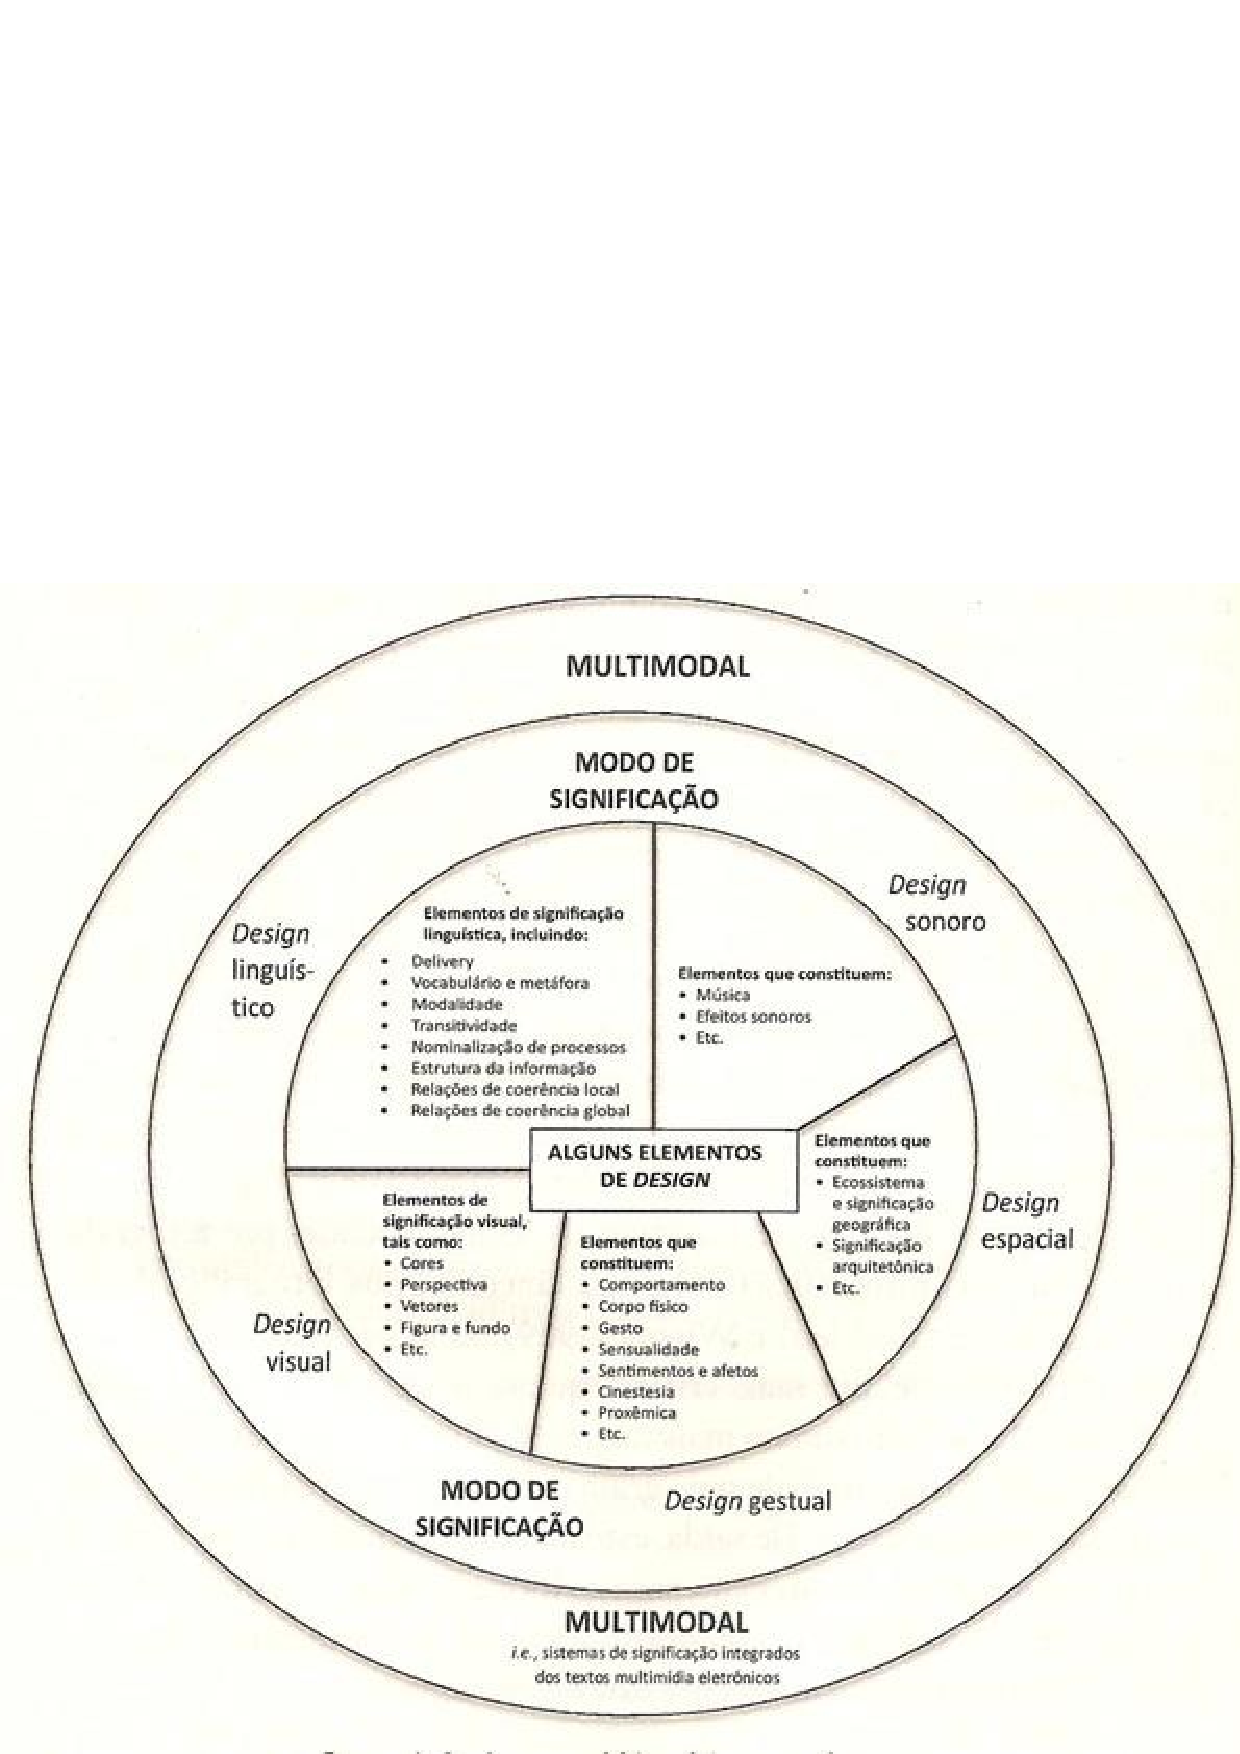
\includegraphics[width=0.8\textwidth]{figure02.png}
 \caption{Jornal do UEADSL -- 2018.}
 \label{fig-fig02}
 \source{\url{https://eventos.textolivre.org/moodle/mod/glossary/showentry.php?courseid=5&eid=95&displayformat=dictionary}.}
\end{figure}

Na sequência realizamos a primeira conferência do Bloco 1: formação docente em debate no evento Seminários teóricos Interdisciplinares do SEMIOTEC (STIS) de 2020, tendo a oportunidade de compartilhar as experiências na formação docente, infâncias e Educação Ambiental. A triangulação das bases, a saber: a inserção ecológica, a participação nos espaços formativos e a linguagem da CNV foram capazes de fortalecer o papel mediador ao pensar a prática e o fazer. Foi necessário mediar diferentes opiniões no chat e ser reflexivo através de questionamentos que possibilitassem uma nova elaboração. A análise das informações resultantes da Inserção Ecológica e pela participação nas formações docente possibilitaram desenhar as oficinas de comunicação e reflexão, que foram realizadas no Brasil e no Uruguai nos anos de 2017 e 2018. As oficinas foram inspiradas no Método da Comunicação Não-Violenta, de \textcite{rosenberg2006}. A educação, as relações proximais e os espaços de conversa(ação) foram o embasamento transversal sistêmico para a realização das oficinas de comunicação e reflexão. A proposta foi organizada em momentos, que não foram isolados, mas montou a engrenagem que (trans)forma e é o todo, que contemplou a criação das oficinas de comunicação e reflexão.

As oficinas foram realizadas em diferentes contextos educativos microssistêmicos, de cinco municípios no Rio Grande do Sul e num município do Uruguai. A estratégia adotada consistiu na produção de informações construídas numa conversa(ação) com os educadores das infâncias de diversos contextos ecológicos microssistêmicos, a saber: 30 são da cidade de Santo Antônio da Patrulha, 30 da cidade de São Lourenço do Sul, 116 da cidade de Rio Grande, 72 da cidade de São José do Norte e 20 da cidade de Treinta y Tres no Uruguai. Nas oficinas de comunicação e reflexão participaram 268 educadores das infâncias, destes 123 são estudantes de graduação, 16 biólogos, 1 professor de matemática, 2 veterinários, 4 guardas florestais de áreas protegidas, 13 professores da Educação Infantil, 7 professores da Creche, 16 professores dos Anos Iniciais, 11 professores de história, 7 enfermeiros, 12 psicólogos, 3 professores de português, 9 professores de educação física, 8 professores da educação do campo, 3 coordenadoras, 2 diretora, 6 monitores, 3 educadores sociais e 22 não responderam. Como não podemos e não devemos fragmentar, já que nosso desejo foi elucidar o todo explicitamos a seguir os estudos, bem como os instrumentos e os procedimentos de cada momento das oficinas de comunicação e reflexão. 

O estudo de cunho qualitativo ao conversar, estar, interagir e propor aos educadores das infâncias a partir das oficinas de comunicação e reflexão ofereceu a possibilidade de reflexão: eu-pessoa, quem sou eu? Quem somos nós? Quais são as práticas educativas realizadas? Foi a maneira de pensar a educação das infâncias para além do contexto escolar: com a comunidade, na educação do campo, nas instituições de acolhimento, nas famílias, dentre outros contextos ecológicos microssistêmicos, em que os educadores atuam, constroem e compartilham conhecimentos com as crianças. 

A ideia foi promover a reflexão e a comunicação a partir de oficinas inspiradas pelo Método de Comunicação Não-Violenta ou também, conhecida como educação compassiva: “para usarmos a CNV, as pessoas com quem estamos nos comunicando não precisam conhecê-la ou mesmo estar movimentadas a se comunicar compassivamente conosco” \cite[p. 24]{rosenberg2006}. A intenção foi contribuir construindo dinâmicas lúdicas, cooperativas e psico(ambientais)corporais com a participação dos educadores das infâncias para que estes se relacionassem com a atuação mediadora e não ficassem estáticos numa educação centrada, enquanto espectadores. Quando referimos a mediação do desenvolvimento humano das infâncias é a partir do conceito dos processos proximais, das interações proximais e de desenvolvimento humano. Por isso, a comunicação foi o eixo central da linguagem ao estabelecer uma conversa atenta com os educadores das infâncias de diferentes contextos ecológicos microssistêmicos.

As construções das oficinas consideraram as especificidades e os interesses temáticos dos educadores das infâncias. Vale mencionar, as mesmas estratégias foram seguidas nos encontros. A proposta inicial foi refletir sobre o “eu-ambiente” e no segundo momento investigar as percepções dos educadores das infâncias para por fim conversar sobre as práticas educativas que estão sendo realizadas nos contextos ecológicos microssistêmicos de suas atuações. As dinâmicas vivenciais foram construídas com os educadores ao conversar sobre o “eu”. Momento que todos tiveram que prestar atenção ao observar os procedimentos, ora adotados para a realização da oficina. Todas as etapas foram construídas com os educadores, no momento inicial da oficina. Os objetivos e os procedimentos, ora individuais, ora coletivos foram possibilidades de refletir sobre as concepções das infâncias, dos vínculos afetivos, dos cuidados e da mediação do desenvolvimento humano nas infâncias ao conversar sobre o “eu-ambiente”. Em seguida, discutimos os sentimentos da CNV alegria, raiva, medo e tristeza. 

A CNV apresenta uma metodologia muito prática cujos eixos são: 1- observação; 2- sentimento; 3- necessidade; 4- pedido \cite{rosenberg2006}. Sendo assim, para propor a CNV é necessário fundamentar nos quatro passos. Depois das oficinas vivenciais, os educadores das infâncias se apropriam, fazem o exercício para a vida, do viver ao ser. Além disso, podem levar as experiências aos contextos em que atuam, tendo a oportunidade de sensibilizar as crianças a usar a CNV. 

As oficinas de comunicação e reflexão seguiram três momentos, a primeira parte da oficina foi buscar estratégias para conhecer o que os educadores pensavam ao investigar as perspectivas deles sobre as infâncias. No momento inicial averiguamos a partir da pergunta: quem sou eu? Como os educadores das infâncias se definem?  Primeiro refletindo o eu-ambiente-pessoas para depois o eu-outro-ambientes. O segundo momento da oficina consistiu em investigar: quem somos nós? Quais são as perspectivas dos educadores das infâncias em âmbito planetário? 

Para a realização da oficina foram mobilizadas diferentes estratégicas psicoeducativas lúdicas e cooperativas denominadas psico(ambientais)corporais. No último momento da oficina investigamos as práticas educativas que são realizadas nos contextos de atuação pelos educadores das infâncias. Tivemos assim, a oportunidade de criar com eles um Projeto de Educação Ambiental das Infâncias. Na continuidade explicativa, apresentamos os instrumentos e os procedimentos: estudos de caso inspiradas no Método da Comunicação Não-Violenta \cite{rosenberg2006} a partir de dinâmicas cooperativas e experienciais, diário de campo, gravações de áudios e a avaliação coletiva ao final das oficinas de comunicação e reflexão. Para a análise dos dados utilizamos o minerador de textos, uma ferramenta de mineração de textos denominada Sobek \cite{epstein2017}.

O minerador de textos extrai as informações de um texto e as representa na forma de um grafo - construções matemáticas para modelar estruturas de informação já, os termos considerados importantes são os nodos e as conexões entre os termos e os nodos – representam as relações entre e com os termos no texto \cite{epstein2017}. A ferramenta Sobek é distribuída gratuitamente e foi desenvolvida pelo Programa de Pós-Graduação em Informática na Educação, na Universidade Federal do Rio Grande do SUL (UFRGS), Brasil.




\section{Produção de informações e encaminhamentos posteriores: capacidade reflexiva de comunicação}\label{sec-producao}

A visão sistêmica é uma forma de olhar o mundo e a teoria Bioecológica do Desenvolvimento Humano \cite{brofen2011}. Portanto, é mais que uma abordagem para as intervenções. A teoria é uma forma de perceber as pessoas e integrar o olhar para as relações, que é sistêmico! Assim, compreendemos um pouco mais sobre as pessoas e os ambientes, percebemos as conexões entre os acontecimentos e que não são e/ou estão isolados, pois eles se modificam ao sofrerem a influência do tempo. 

\textcite{brofen2011} defendeu que o desenvolvimento humano se dá por meio da interação permanente e recíproca do indivíduo e do contexto. É a compreensão sobre as dimensões que influenciam a constituição de cada criança enquanto um misto entre contexto, os processos, a personalidade e o tempo, ou seja, indivíduos-contextos numa vertente sistêmica da vida, o viver é a base relacional da vertente sistêmica. Como se concebe a linha sistêmica? Significa entender que tudo está relacionado, que não temos como compreender a pessoa de forma dissociada do contexto, pois ela é contexto/ natureza, e estes ambientes se organizam em forma de sistemas. Sistemas são níveis de entendimento, as dimensões em que podemos apreender sobre o mundo e metamorfosear das/pelas relações que estão implicadas e são indissociáveis pelo olhar bioecológico das crianças e dos educadores nos múltiplos contextos ecológicos microssistêmicos. As dimensões podem ser acompanhadas na metamorfose de uma borboleta, conforme \Cref{fig-fig03}. 

\begin{figure}[h!]
 \centering
 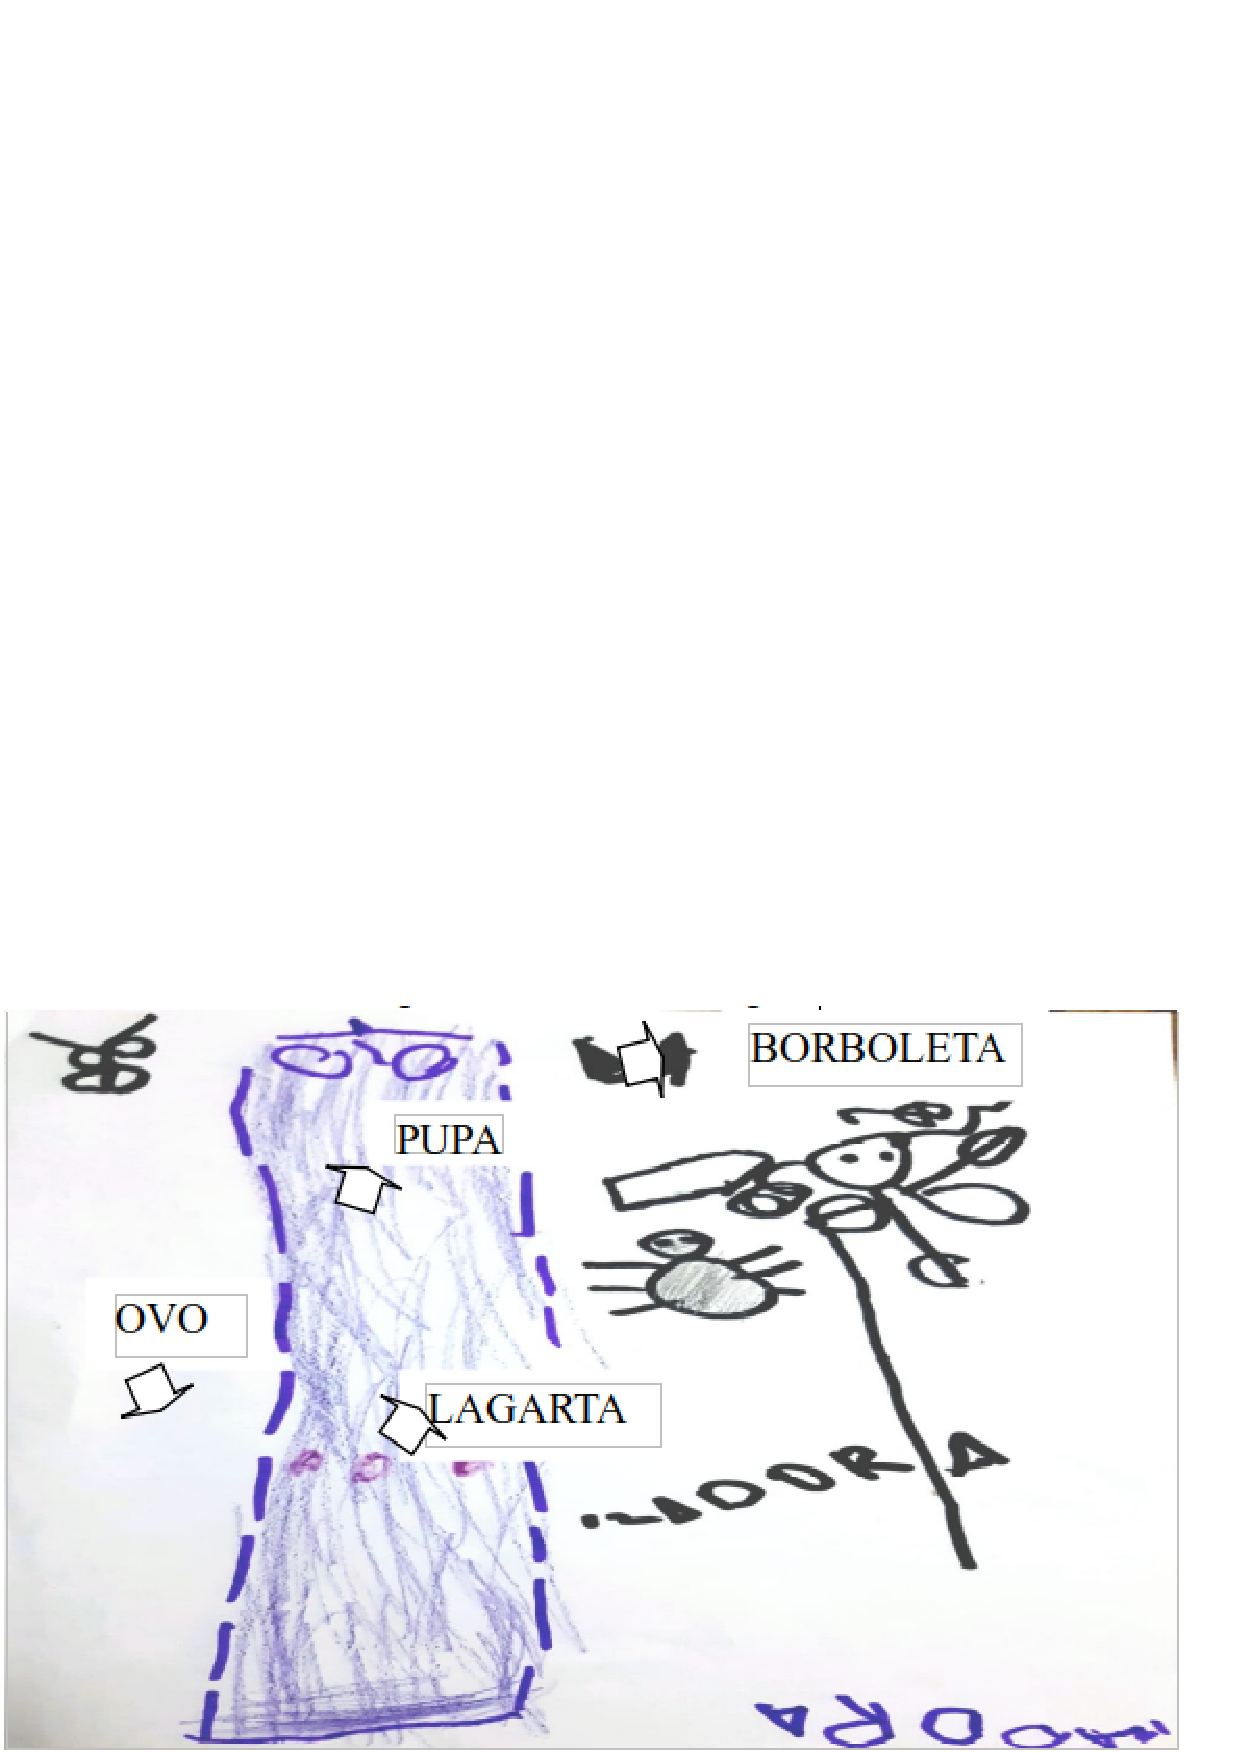
\includegraphics[width=0.7\textwidth]{figure03.png}
 \caption{Olhar bioecológico.}
 \label{fig-fig03}
 \source{Isadora, 5 anos.}
\end{figure}


Na delicadeza expressa pelos traços que contornam a metamorfose, podemos perceber as trans(formações) do ciclo da vida, sempre acompanhadas pelo olho, que é do reino animal. Chamamos a atenção para os olhos que estão (são) em todas as dimensões, representadas no desenho feito pela Isadora e em sua interpretação das lentes. O foco da lente não pode ser fragmentado em partes, é necessário olhar e contemplar os quatro estágios da borboleta, metamorfosear a auto(trans)forma(ação) em sua totalidade, pelas nuances dos vários olhos da borboleta, e que também é acompanhado pelo olhar da criança. Isadora desenhou a borboleta pela representação de uma pessoa com as asas e os olhos. Interessante perceber as similaridades para além dos olhos. As borboletas, assim como os humanos precisam desta engrenagem: pessoa, processo, tempo e contexto e isso vem ao encontro de outra imagem construída pela Mayara (\Cref{fig-fig04}): 

\begin{figure}[h!]
 \centering
 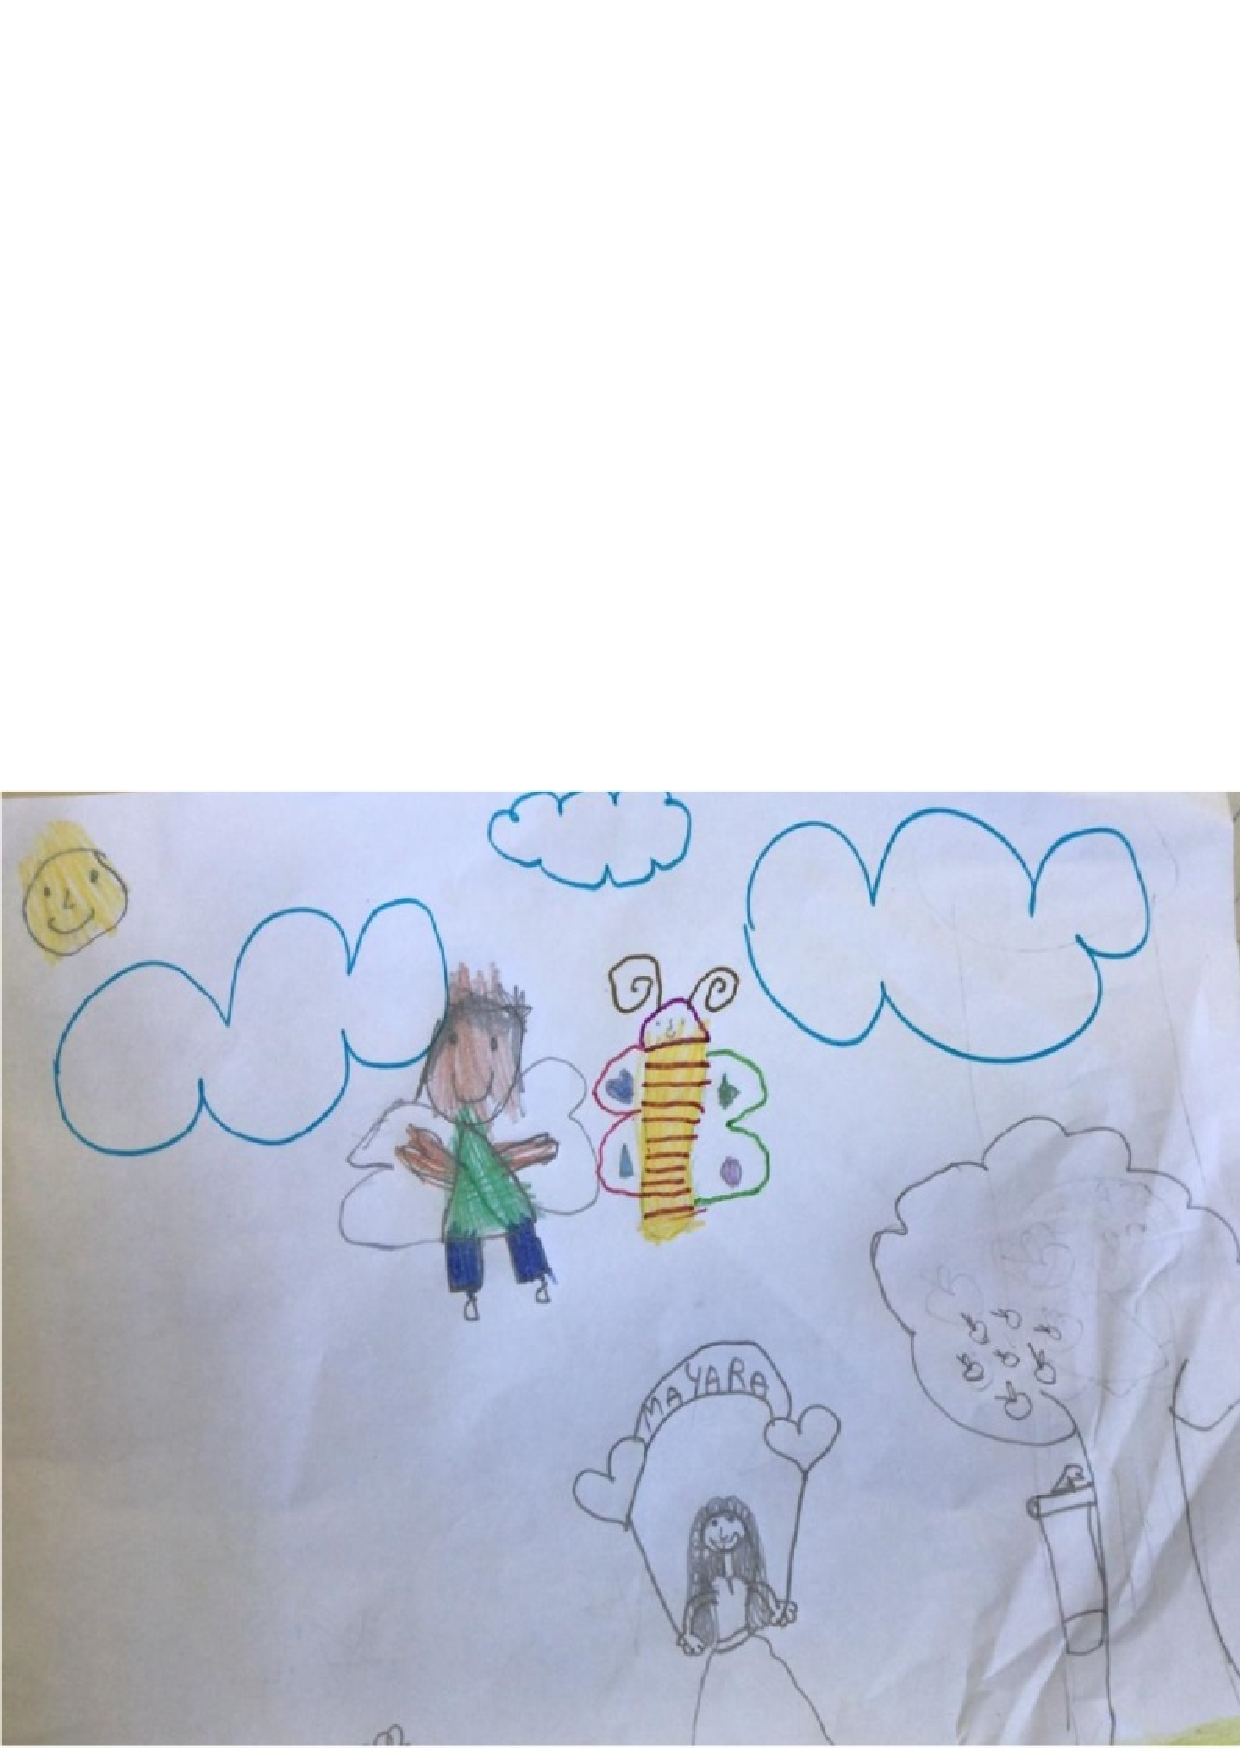
\includegraphics[width=0.6\textwidth]{figure04.png}
 \caption{Metamorfosear os elementos: PPCT.}
 \label{fig-fig04}
 \source{Mayara, 9 anos.}
\end{figure}

As crianças destacaram o olhar bioecológico para a investigação bioecológica nas/das (com as) infâncias e foram elas que enfatizaram a integralidade dos elementos, desde os primeiros passos da Inserção Ecológica. Chamamos a atenção para outro desenho, que integra a lente bioecológica e o olhar bioecológico, que apesar de não serem iguais têm similaridades. O que é possível confirmar pela representação da imagem, que evidencia as particularidades contidas nos elementos. A lente bioecológica é a forma como tentamos buscar o viés bioecológico, que é algo para além daquilo que o pesquisador interpreta. No desenho é imaginado pela lupa, ao centro e ao entorno acompanhamos os elementos indissociáveis: pessoa, processo, tempo e contexto. Neste mesmo desenho podemos observar que as cores se misturam e representam o metamorfosear relacional, sem fragmentações do olhar. O olhar bioecológico que integra a lente pode ser acompanhado na imagem, que é representada pela lupa, conforme \Cref{fig-fig05}. 

\begin{figure}[h!]
 \centering
 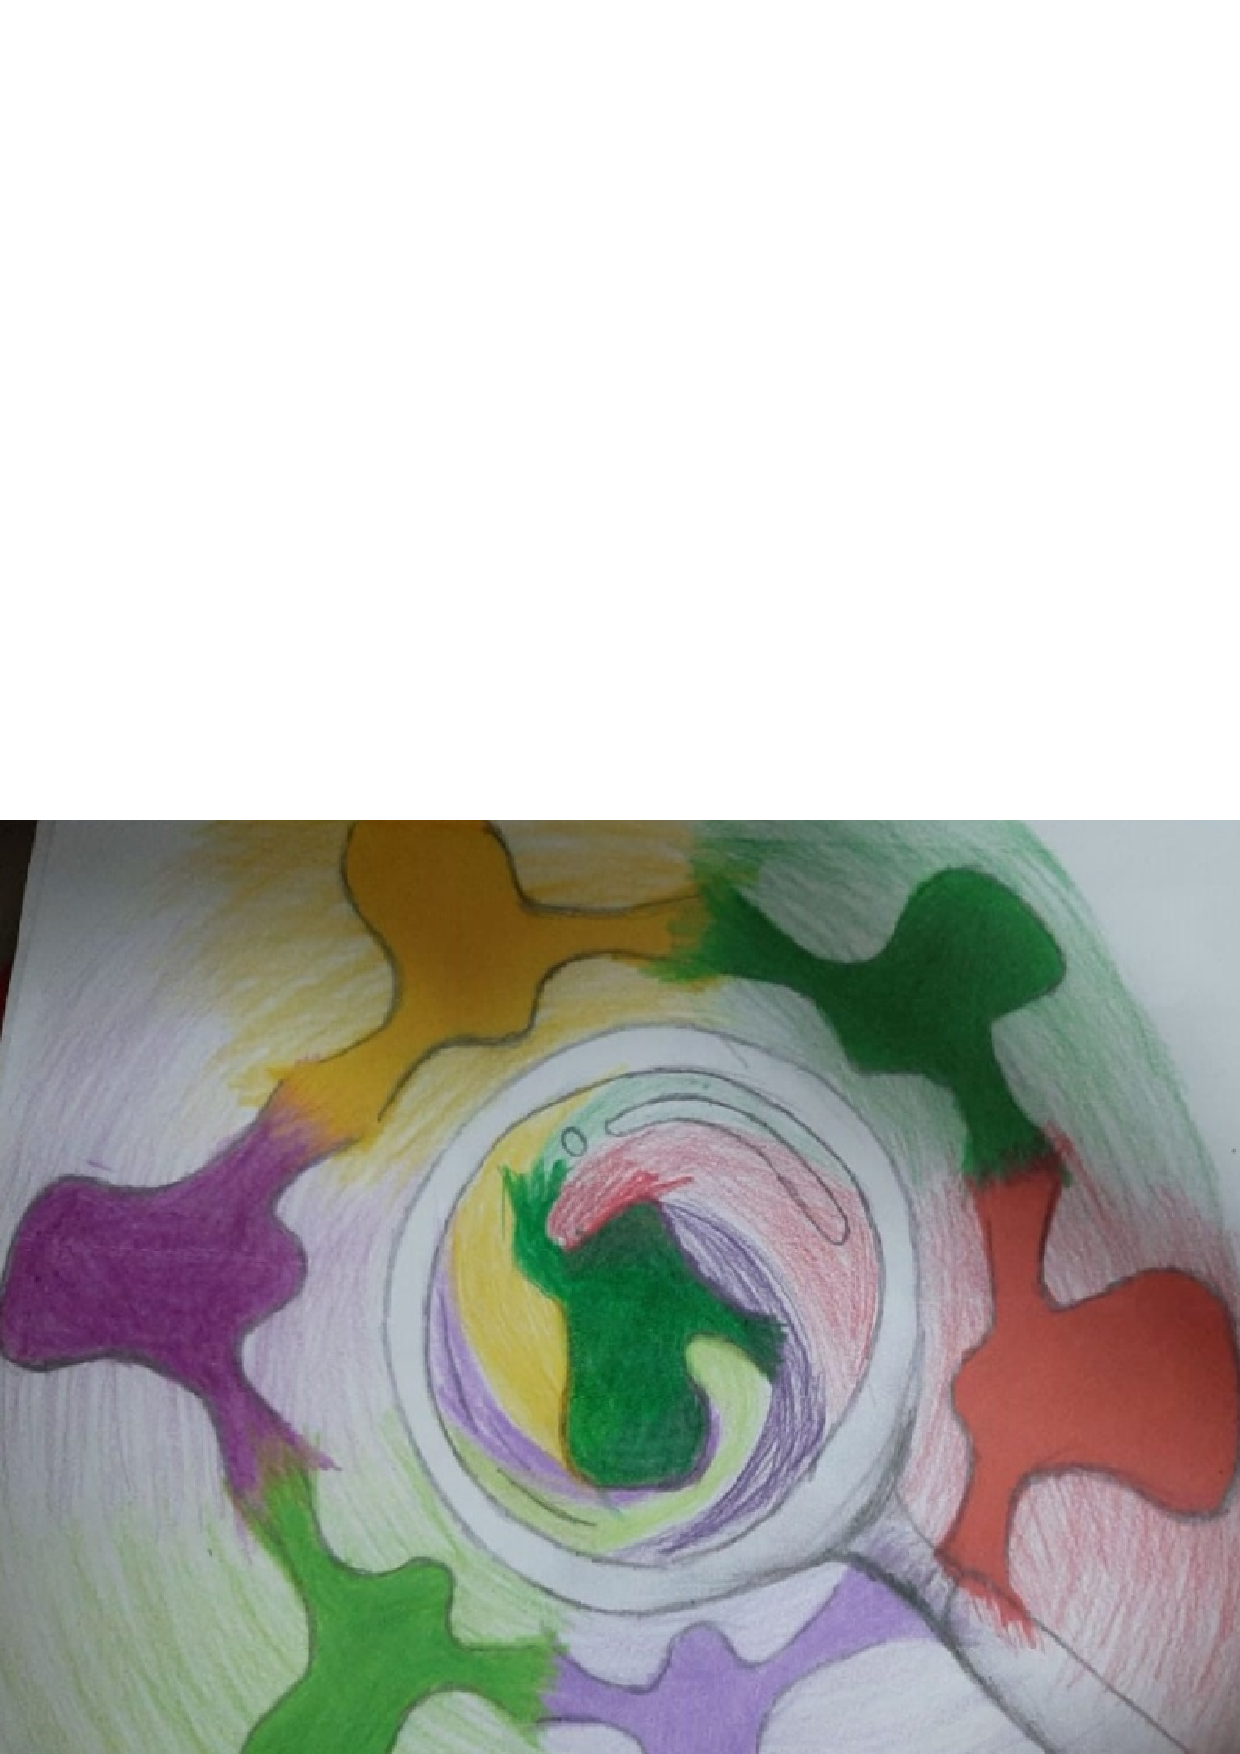
\includegraphics[width=0.6\textwidth]{figure05.png}
 \caption{Eu-ambiente-processo-tempo.}
 \label{fig-fig05}
 \source{Felipe, 15 anos.}
\end{figure}


Numa tentativa de síntese, a perspectiva ambiental sistêmica está representada na imagem, sendo a possibilidade para a construção de uma percepção integrada dos componentes que vão do micro ao macrossistema e/ou vice-versa. Além disso, interligam os aspectos PPCT (pessoa-processo-contexto-tempo) na pesquisa. Aproveitamos o ensejo para apresentar o desenho da Isadora, que muito mais do que contextualizar a Bioecologia do Desenvolvimento Humano com a Vertente Sistêmica da Educação Ambiental evidencia as dimensões intrínsecas PPCT, que estão (são) interconectados como um espiral infinito, em que o movimento da estrutura ondulada apresenta a indissociabilidade dos elementos bioecológicos, que oras vai e em outros retorna. Essas interconexões podem ser visualizadas com a \Cref{fig-fig06}.

\begin{figure}[h!]
 \centering
 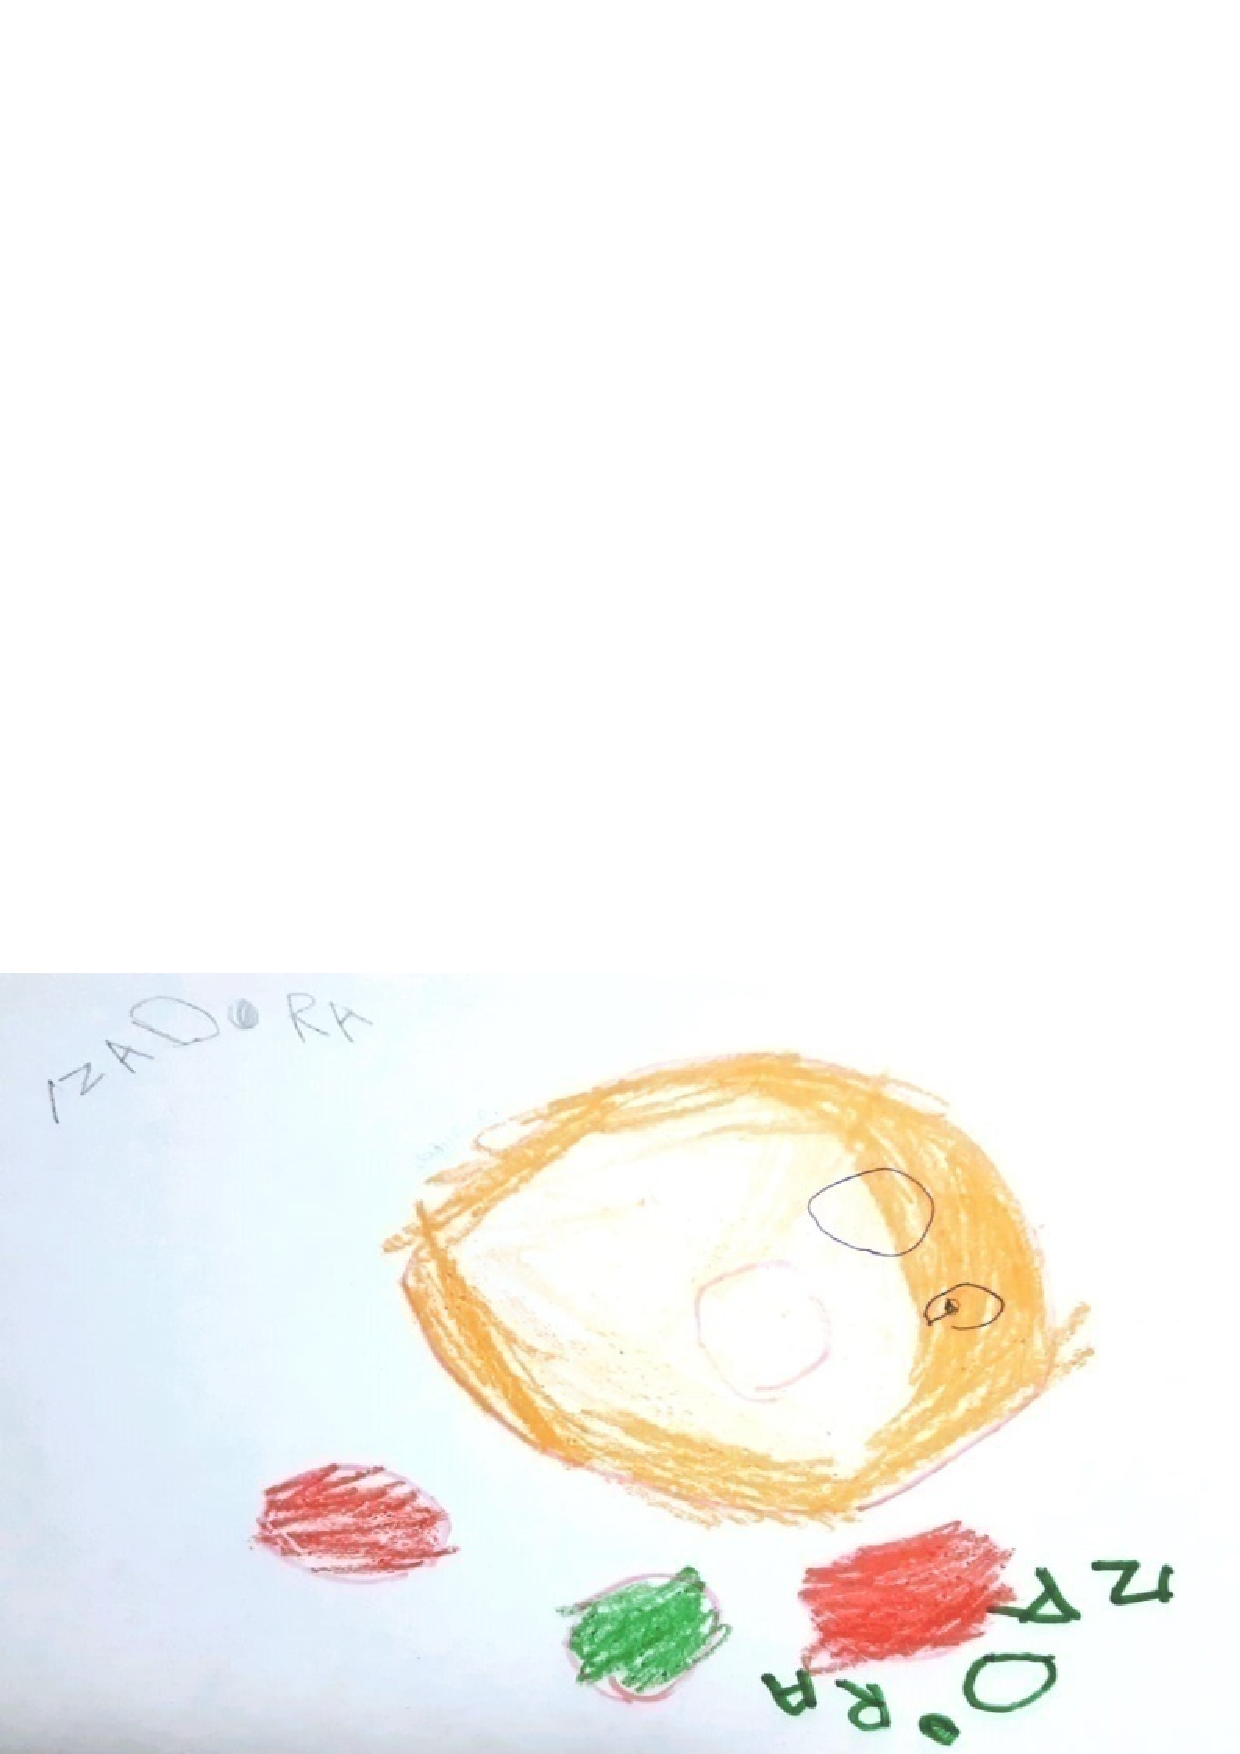
\includegraphics[width=0.6\textwidth]{figure06.png}
 \caption{Interconexões bioecológicas.}
 \label{fig-fig06}
 \source{Isadora, 4 anos.}
\end{figure}

As interconexões apresentadas com o desenho de Isadora subsidiaram o olhar sistêmico dos educadores ambientais das infâncias na educação das crianças em múltiplos contextos ecológicos microssistêmicos para o desenvolvimento humano nas infâncias \cite{piske2019}. As perspectivas sistêmicas das dimensões bioecológicas foram a mola propulsora das junções dos desenhos, a chave holística da Bioecologia do Desenvolvimento Humano \cite{brofen2011} com a Biologia do Conhecer \cite{maturana2011} pelas bases metodológicas: a Inserção Ecológica e a formação docente. Quando nos referimos à chave holística é para apresentar o interstício conceitual-metodológico da pesquisa. 

O olhar bioecológico expresso pelas crianças nos desenhos possibilitou o embasamento bioecológico das infâncias. Salientamos as preposições nas/das (para/com as) infâncias que estão presentes no estudo têm a intenção trazer e destacar a força das díades e grupos relacionais com duas ou mais pessoas na educação das crianças, o que possibilitou apresentar a estratégia metodológica na perspectiva sistêmica ambiental. Salientamos que educação é sempre educação como um direito essencial as crianças nos ambientes educativos \cite{piske2019}. 

Nas oficinas de comunicação e reflexão participaram 268 educadores das infâncias, conforme já mencionado. A produção de informações construídas com os educadores das infâncias ao participarem das oficinas de comunicação e reflexão foi um momento de compreender as perspectivas dos educadores das infâncias. Com a análise dos dados, percebemos uma confusão acerca dos papéis que assumem os educadores das infâncias nos contextos ecológicos microssistêmicos, conforme apresenta a mineração de texto com a ferramenta Sobek, conforme \Cref{fig-fig07}:

\begin{figure}[h!]
 \centering
 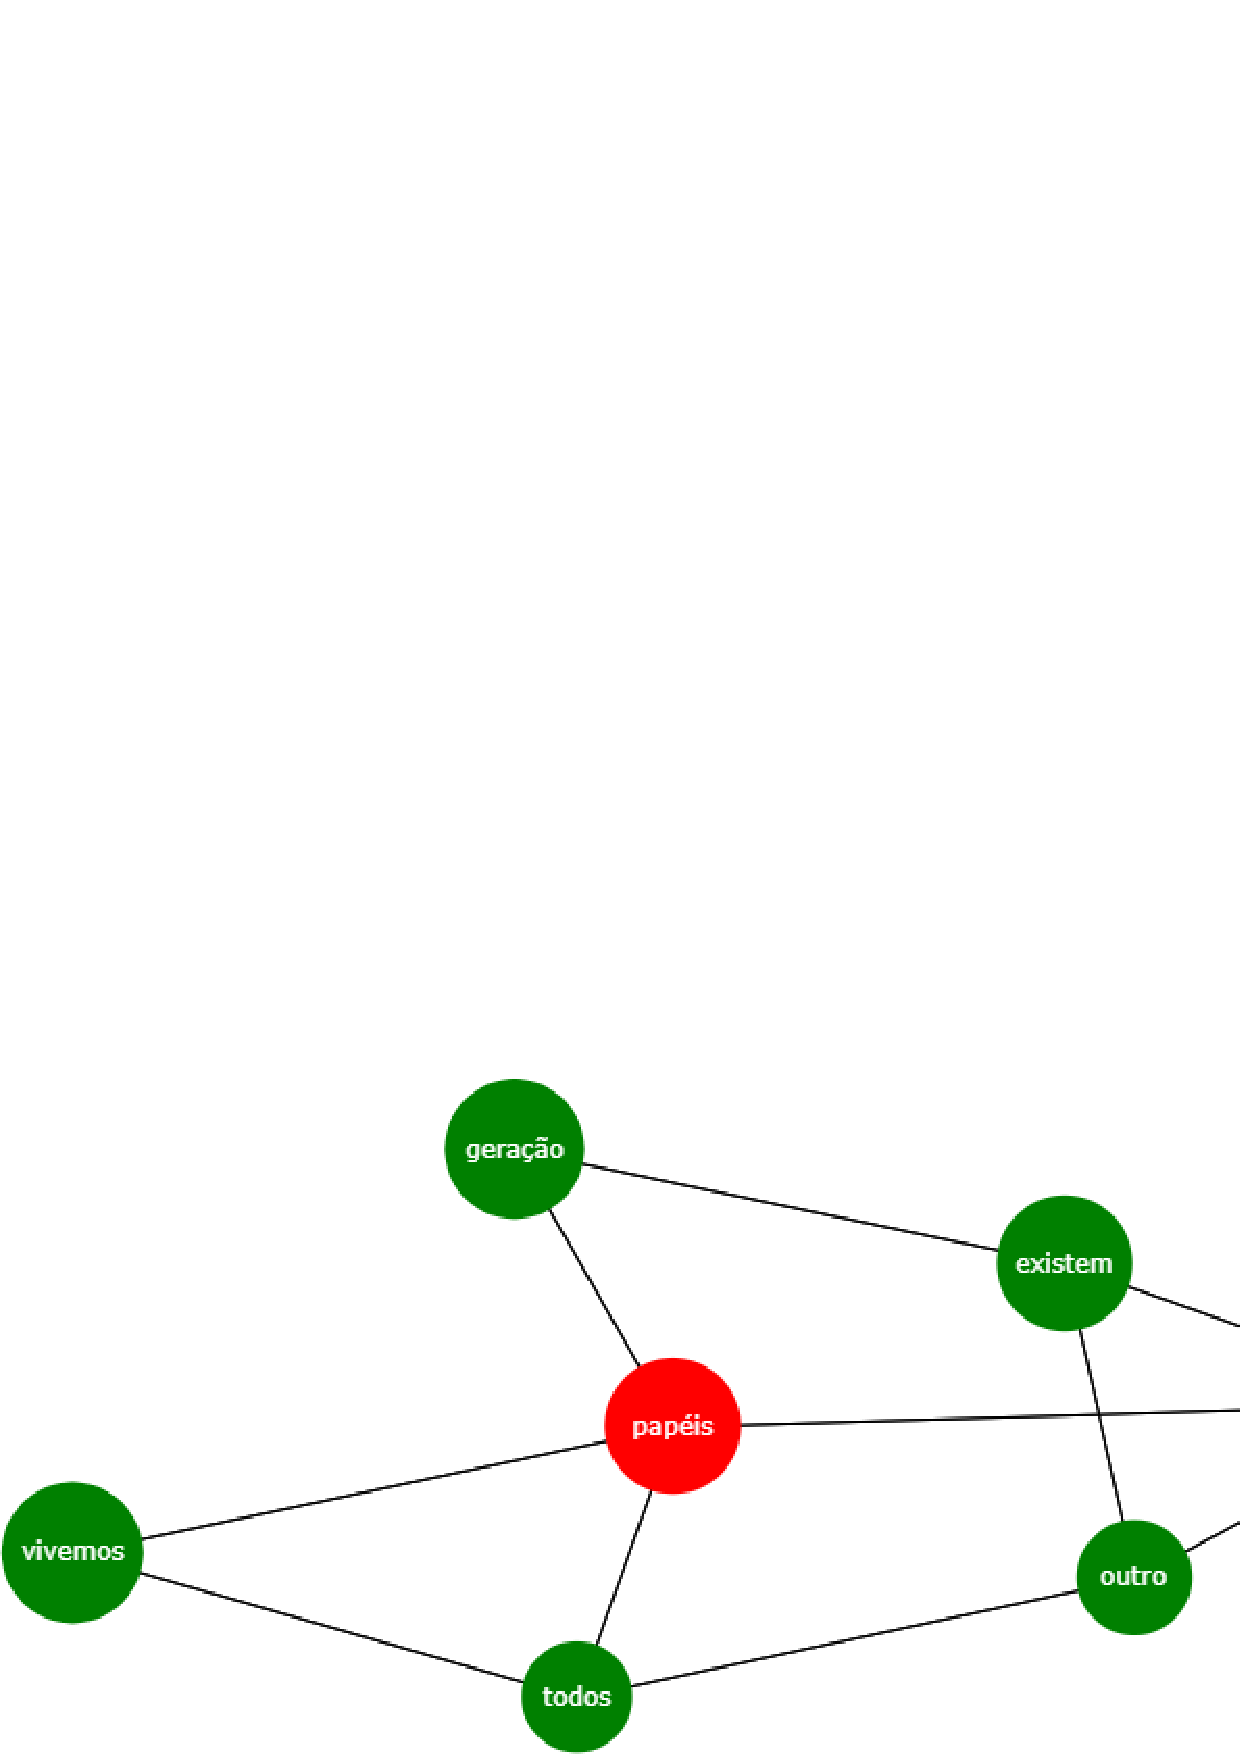
\includegraphics[width=0.8\textwidth]{figure07.png}
 \caption{Grapho papéis dos educadores das infâncias -- gerado no Sobek.}
 \label{fig-fig07}
 \source{Desenvolvido pelas autoras.}
\end{figure}


No decorrer do artigo, serão retomadas as “confusões” acerca dos papéis dos educadores das infâncias, que não são somente acerca das questões, mas das responsabilidades que são colocadas ao(s) outro(s) e para as gerações futuras. Importante retomar alguns dados importantes acerca da Inserção Ecológica e da participação nos espaços formativos. Fato que causou bastante surpresa é que 54 EI baseiam os discursos na lógica da punição e recompensa, o que a CNV quer desconstruir. A \Cref{fig-fig08} ilustra a punição para a criança obedecer: 

\begin{figure}[h!]
 \centering
 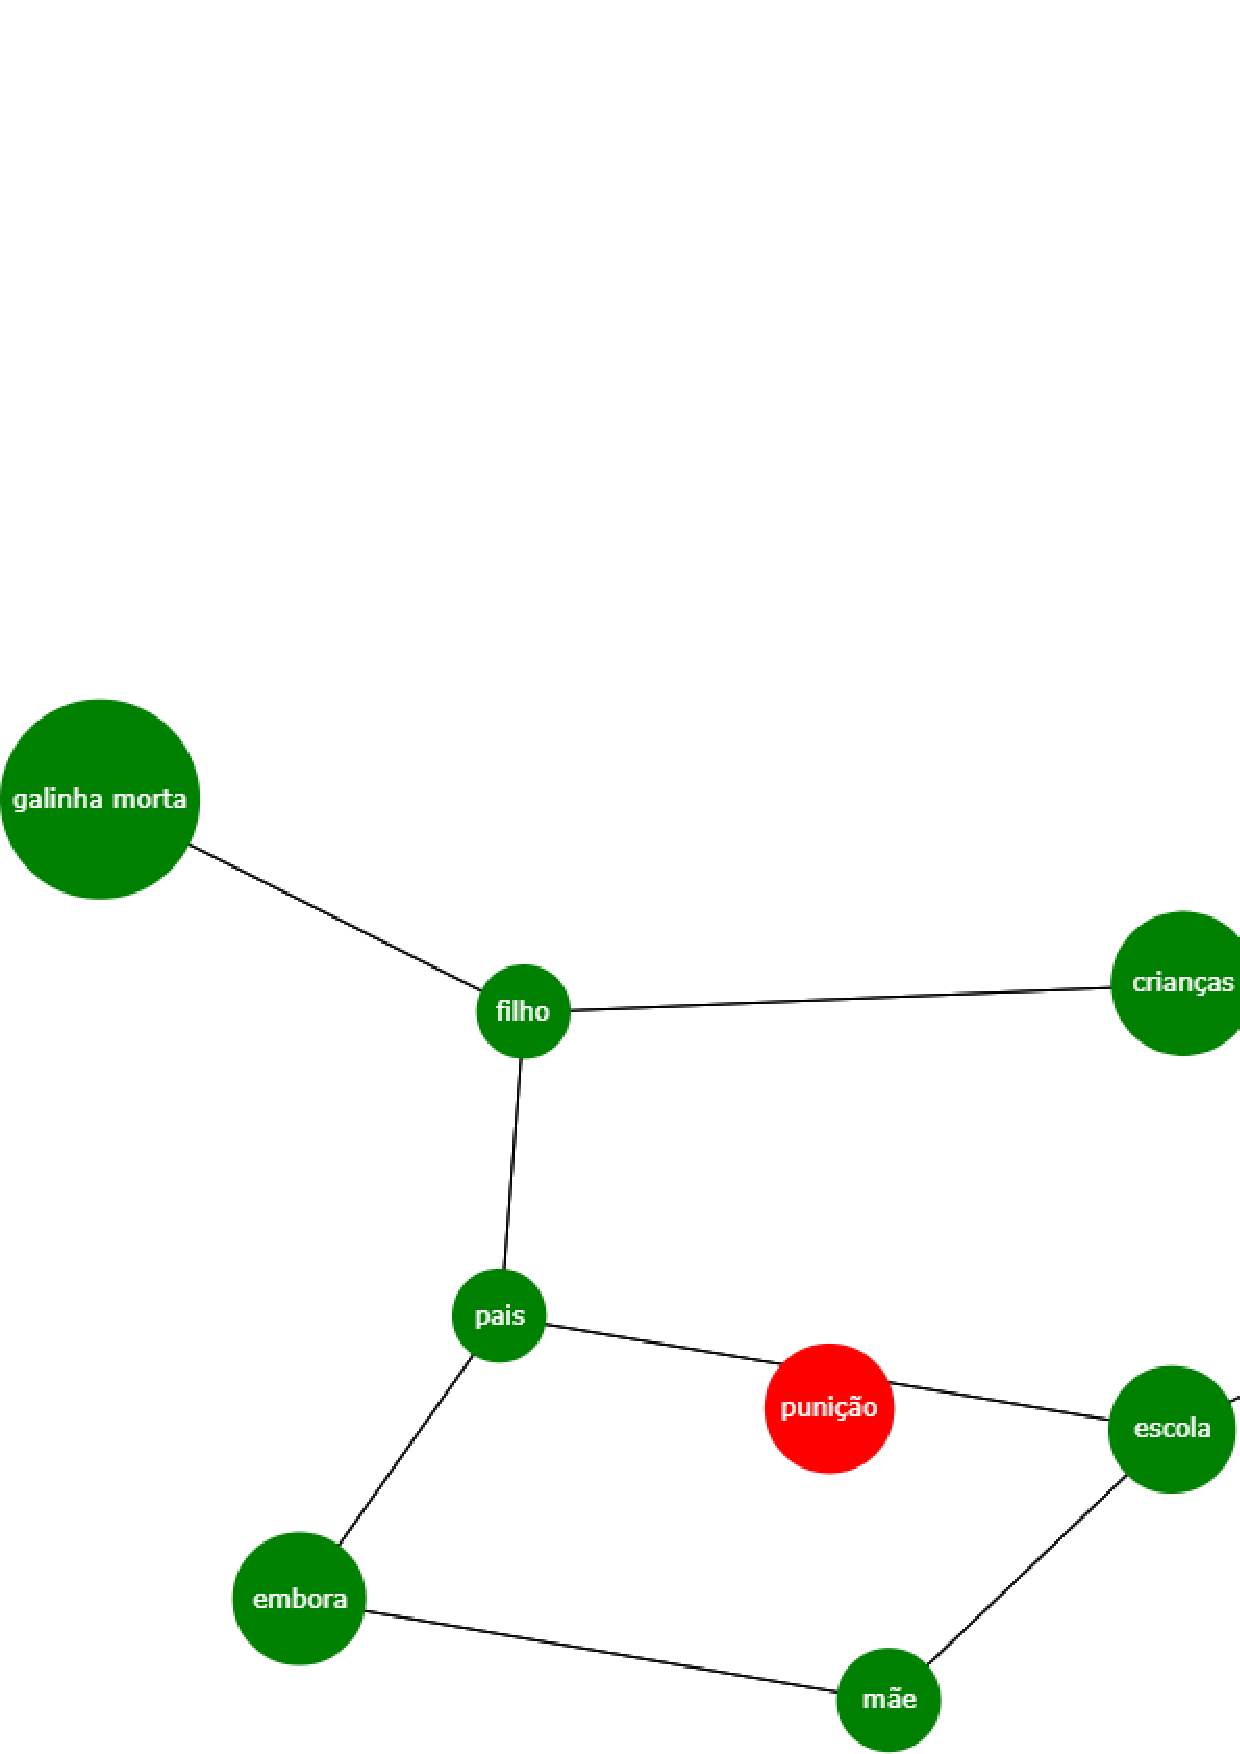
\includegraphics[width=0.8\textwidth]{figure08.png}
 \caption{Grapho papéis dos educadores das infâncias -- gerado no Sobek.}
 \label{fig-fig08}
 \source{Desenvolvido pelas autoras, 2020.}
\end{figure}


No trecho a seguir fica evidente o castigo psicológico apontado num curso de formação. A alternativa proposta pelo educador das infâncias para a educação das crianças, para que aprendam a obedecer evidencia essas singularidades:

\begin{quote}
A educadora Maria\footnote{Na pesquisa vamos adotar nomes fictícios para preservar as identidades dos educadores.} disse que as crianças não respeitam, ela se sente cansada, o turno de trabalho é exaustivo, com crianças correndo, sem limites e quando chega em casa os filhos também querem aprontar mas, educar os meus filhos é fácil. Logo, citou um exemplo, um dos filhos dela vivia fugindo para a rua foi assim até o dia em que ela percebeu que tinha uma galinha morta na esquina, pegou o filho pela mão e fez tocar na galinha morta para que a criança visse o que acontece quando fogem dos pais, morre. Meu filho eu sei ensinar agora, nunca mais ele fugiu de perto de mim. Mas, as crianças que eu cuido não posso fazer isso do contrário, elas iam aprender (Diário de campo, agosto de 2017). 
\end{quote}

Percebemos uma distorção no papel do educador, da identidade de quem cuida, a identidade do cuidado. Alguns educadores das infâncias não se reconhecem educadores na afetividade, mencionam que na maioria das vezes, é necessário impor para que as crianças possam obedecer. Afirmam que o papel dos pais é educar e da escola é ensinar. É necessário entender que o cuidado e a educação precisam ser coletivos e recíprocos. Não apenas é responsabilidade da escola nem só das famílias. Na oportunidade trouxemos outro relato, Tinah trabalha numa escola: “como é difícil ensinar as crianças. Os pais não são presentes na escola, só conseguimos quando colocamos bilhete na agenda- vai ter festa com comida” (Diário de campo, novembro de 2017). Rapidamente, Duda interrompe e fala:

\begin{quote}
Vou contar algo que aconteceu na minha escola, mas é um alerta para todos nós. Neste ano, recebemos uma aluna que diariamente chegava à escola com piolhos e os pais não eram presentes, embora frequentemente fossem enviados bilhetes na agenda. A menina ainda não sabia ler. Um dia, a professora já sem saber o que fazer disse para a criança amanhã, tu só entras na escola com tua mãe. No outro dia a criança não foi a aula. Após três dias, no horário da saída chega essa mãe para conversar, a professora explica a situação e alerta que precisou chamar o Conselho Tutelar. A mãe dessa criança não sabe ler e trabalha na cebola. A mãe vai embora. No outro dia, a criança chega na escola com os cabelos raspados (...). A criança foi para a instituição de acolhimento, mais uma vez (Diário de campo, 2017).
\end{quote}

As anotações nos diários de campo e as gravações, posteriormente transcritas foram fundamentais para a apresentação das informações. Nas oficinas, os educadores tiveram a oportunidade de conversar e refletir coletivamente sobre as ações ao (re)pensar suas atuações. Percebemos equívocos sobre a concepção de educação das crianças e as dicotomias entre o educar e o ensinar. Nas expressões dos educadores das infâncias era nítido as tentativas de responsabilizar alguém e até mesmo uma situação, sem problematizar suas atuações com os outros e nos ambientes: eu-ambiente. A conversa ao mobilizar a reflexão sobre o “eu” ambiente causou espanto com os educadores, muitos relataram que estavam imaginando uma oficina teórica. Quais são as compreensões acerca da educação das crianças? 

Tivemos a oportunidade de conversar com os educadores sobre a educação das crianças a partir da Educação Ambiental das Infâncias, temática que emergiu nas rodas de comunicação e reflexão. Os EI em sua maioria relacionavam a Educação Ambiental apenas com a separação do lixo. Aproveitamos o ensejo para questionar: como construir um Projeto de Educação Ambiental das Infâncias? Esse foi um importante momento da oficina de comunicação e reflexão, em que retomamos as atividades construídas coletivamente, possibilidade que os educadores das infâncias apontaram suas perspectivas acerca da educação das crianças. A questão da conversa é a necessidade de todos, foi o esteio para mensurar as perspectivas e chegar ao emaranhado de estratégias para a conversa(ação) do texto com a ferramenta Sobek, a seguir podemos acompanhar pela \Cref{fig-fig09}. 

\begin{figure}[h!]
 \centering
 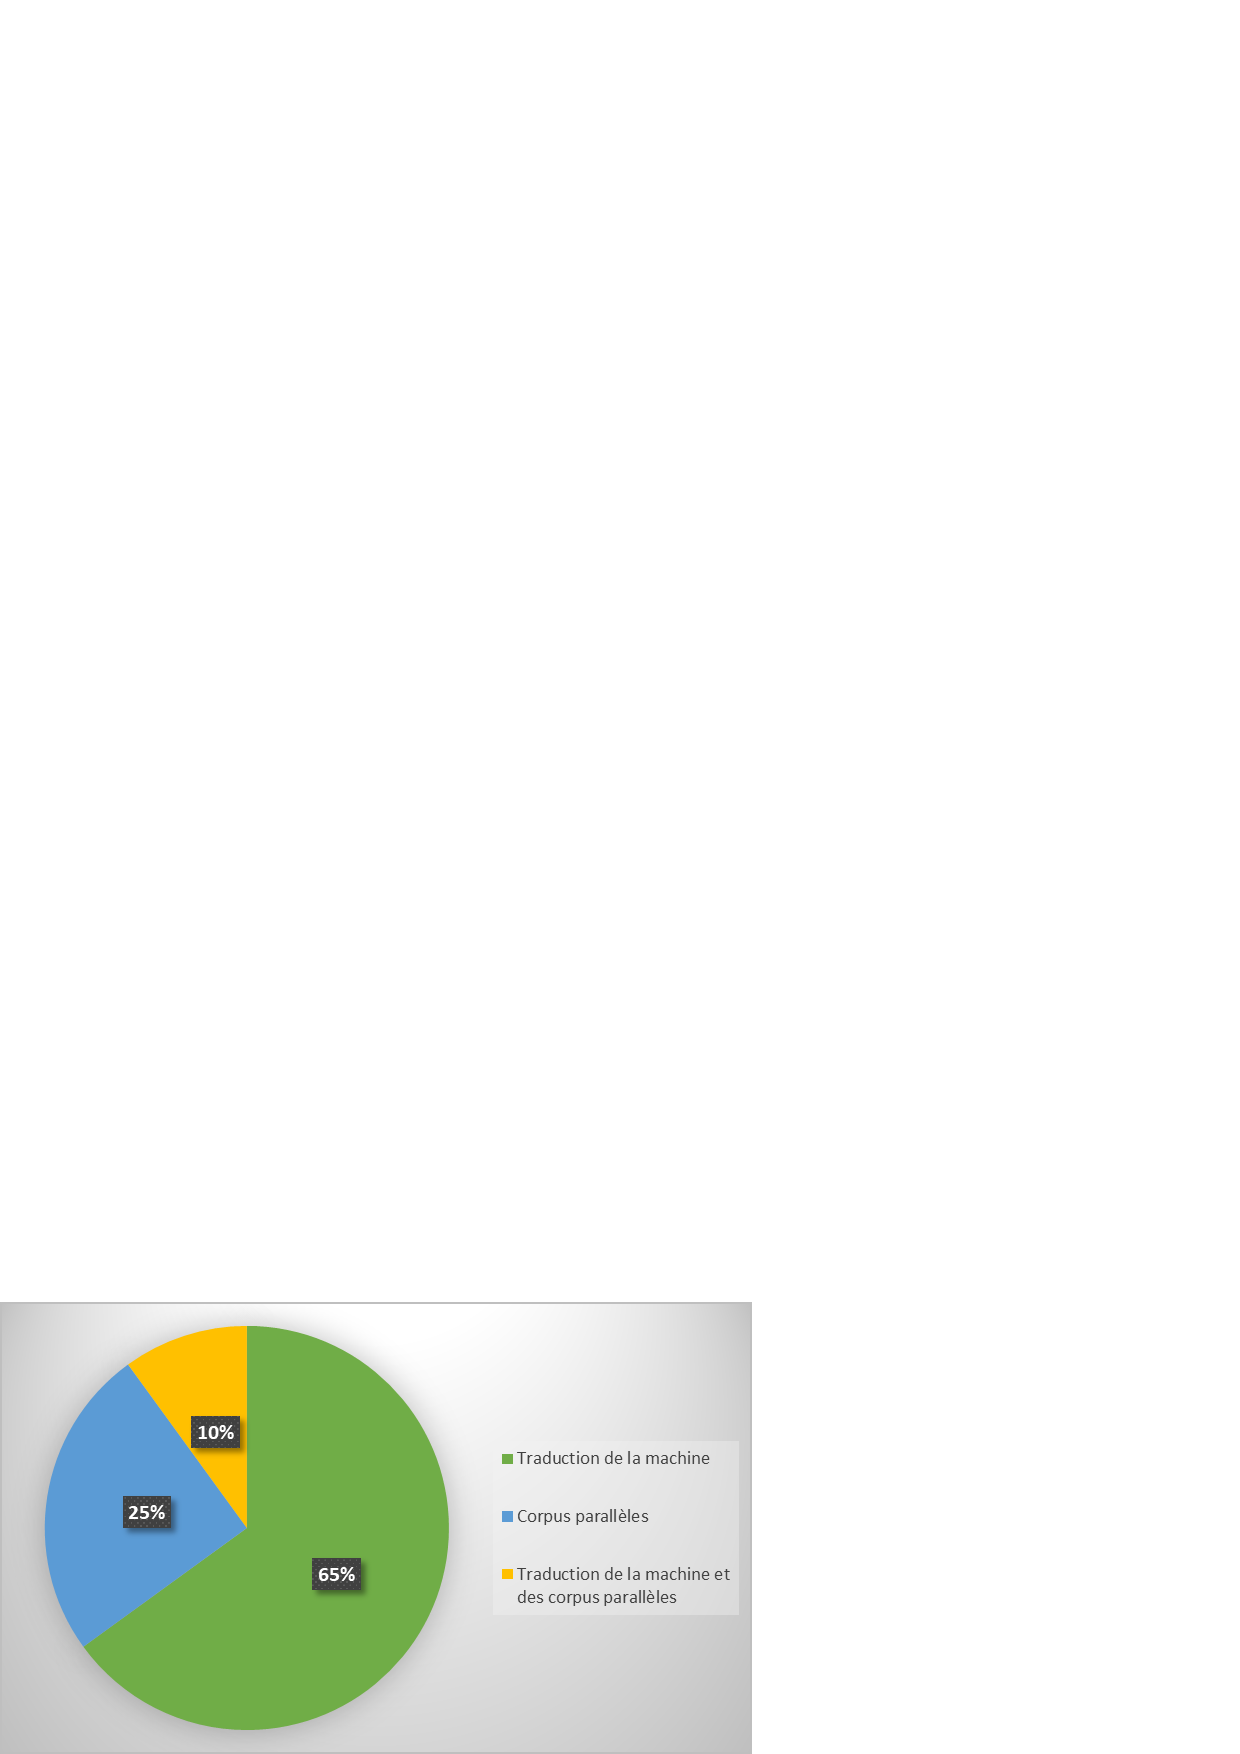
\includegraphics[width=0.8\textwidth]{figure09.png}
 \caption{Grapho perspectivas dos educadores das infâncias -- gerado no Sobek.}
 \label{fig-fig09}
 \source{Desenvolvido pelas autoras.}
\end{figure}

O ponto central mencionado pelos educadores das infâncias foi a carência na formação docente a partir de temáticas escolhidas por eles. Foram relacionadas as dificuldades encontradas pela escassez de espaços formativos, inclusive mencionamos a falta de um ambiente para comunicação e reflexão a partir das experiências. Nessa ocasião os participantes solicitaram que as formações fossem vivenciais e envolvessem práticas à distância e presenciais, resultados que emergiram na avaliação das oficinas. A possibilidade de pensar a educação como processo das relações proximais e a importância do tempo das trajetórias educativas auxilia a refletir sobre as perspectivas dos educadores das infâncias pela produção de informações.

De forma geral, as inserções e a participação nos espaços formativos permitiram observar de forma sistêmica, os aspectos psico(ambientais)corporais, tecnológicos e lúdicos paralelamente com os demais elementos que estão presentes nos contextos ecológicos microssistêmicos. Tais elementos carecem de compreensão mais abrangente.


\section{Considerações finais}\label{sec-consideracoes}
A existência humana com a conjuntura sistêmica das estratégias possibilitou integrar as quatro dimensões na pesquisa: pessoa-processo-tempo-contexto. Com isso, se constituíram as interações necessárias para promover o olhar bioecológico, essencial para investigar quais são as práticas educativas ambientais nos contextos ecológicos microssistêmicos. Com esse estudo conseguimos responder ao objetivo proposto e comprovamos que as dimensões estão relacionadas sistemicamente, sendo portanto, impossível separar os elementos. Em nenhum momento buscamos fazer uma análise dos desenhos, mas as representações foram interpretadas pelas crianças nas construções com os educadores das infâncias nos múltiplos contextos de atuação, momento registrado no diário de campo acerca das percepções.

Cabe destacar que as conversas com os educadores das infâncias mobilizaram saberes e concepções sobre o fazer docente e suas práticas educativas ambientais com as crianças. É perceptível que algumas experiências ainda estão restritas a um olhar mais conservacionista e de preservação da natureza. Por outro lado, os relatos sobre a complexidade da educação e da atuação diante das diferentes infâncias evidenciaram uma perspectiva sistêmica sobre as relações sociais e o reconhecimento da relevância do papel desses educadores para a Educação Ambiental em contextos ecológicos diversos.

Concluímos que a Educação Ambiental na formação dos educadores das infâncias e no mapa bioecológico das crianças são aspectos a serem considerados no processo relacional das experiências em contextos. O olhar bioecológico mobilizou atuações, sensibilizou saberes ambientais e estabeleceu uma relação sistêmica de compreensão bioecológica das infâncias como desenvolvimento humano. Esta, não consistiu apenas em relatar as dificuldades, mas entender as crenças e as raízes de percepções de si mesmo e de responsabilidades. Consequentemente os educadores ambientais das infâncias, a partir de reflexões compartilhadas puderam transformar práticas educativas alterando os comportamentos e atitudes nos seus contextos ecológicos microssistêmicos. 


\section*{Agradecimento}
Coordenação de Aperfeiçoamento de Pessoal de Ensino Superior – CAPES pelo financiamento da pesquisa que originou o artigo.



\printbibliography
\end{document}
